% !TEX root = main.tex

\subsection{上板}
\qquad 几条代表性指令的Basys3板结果如下,其他指令结果见具体实现。从左到右从上到下四幅图依次是:当前/下条PC、rs寄存器地址/值、rt寄存器地址/值、ALU结果输出/DB总线数据。可以看见上板结果与前面仿真分析的结果相同,成功证明了程序的正确性。
\begin{enumerate}
    \item 0x00: \verb'addiu $1, $0, 8'
    \begin{figure}[H]
    \centering
    \begin{tabular}{cc}
    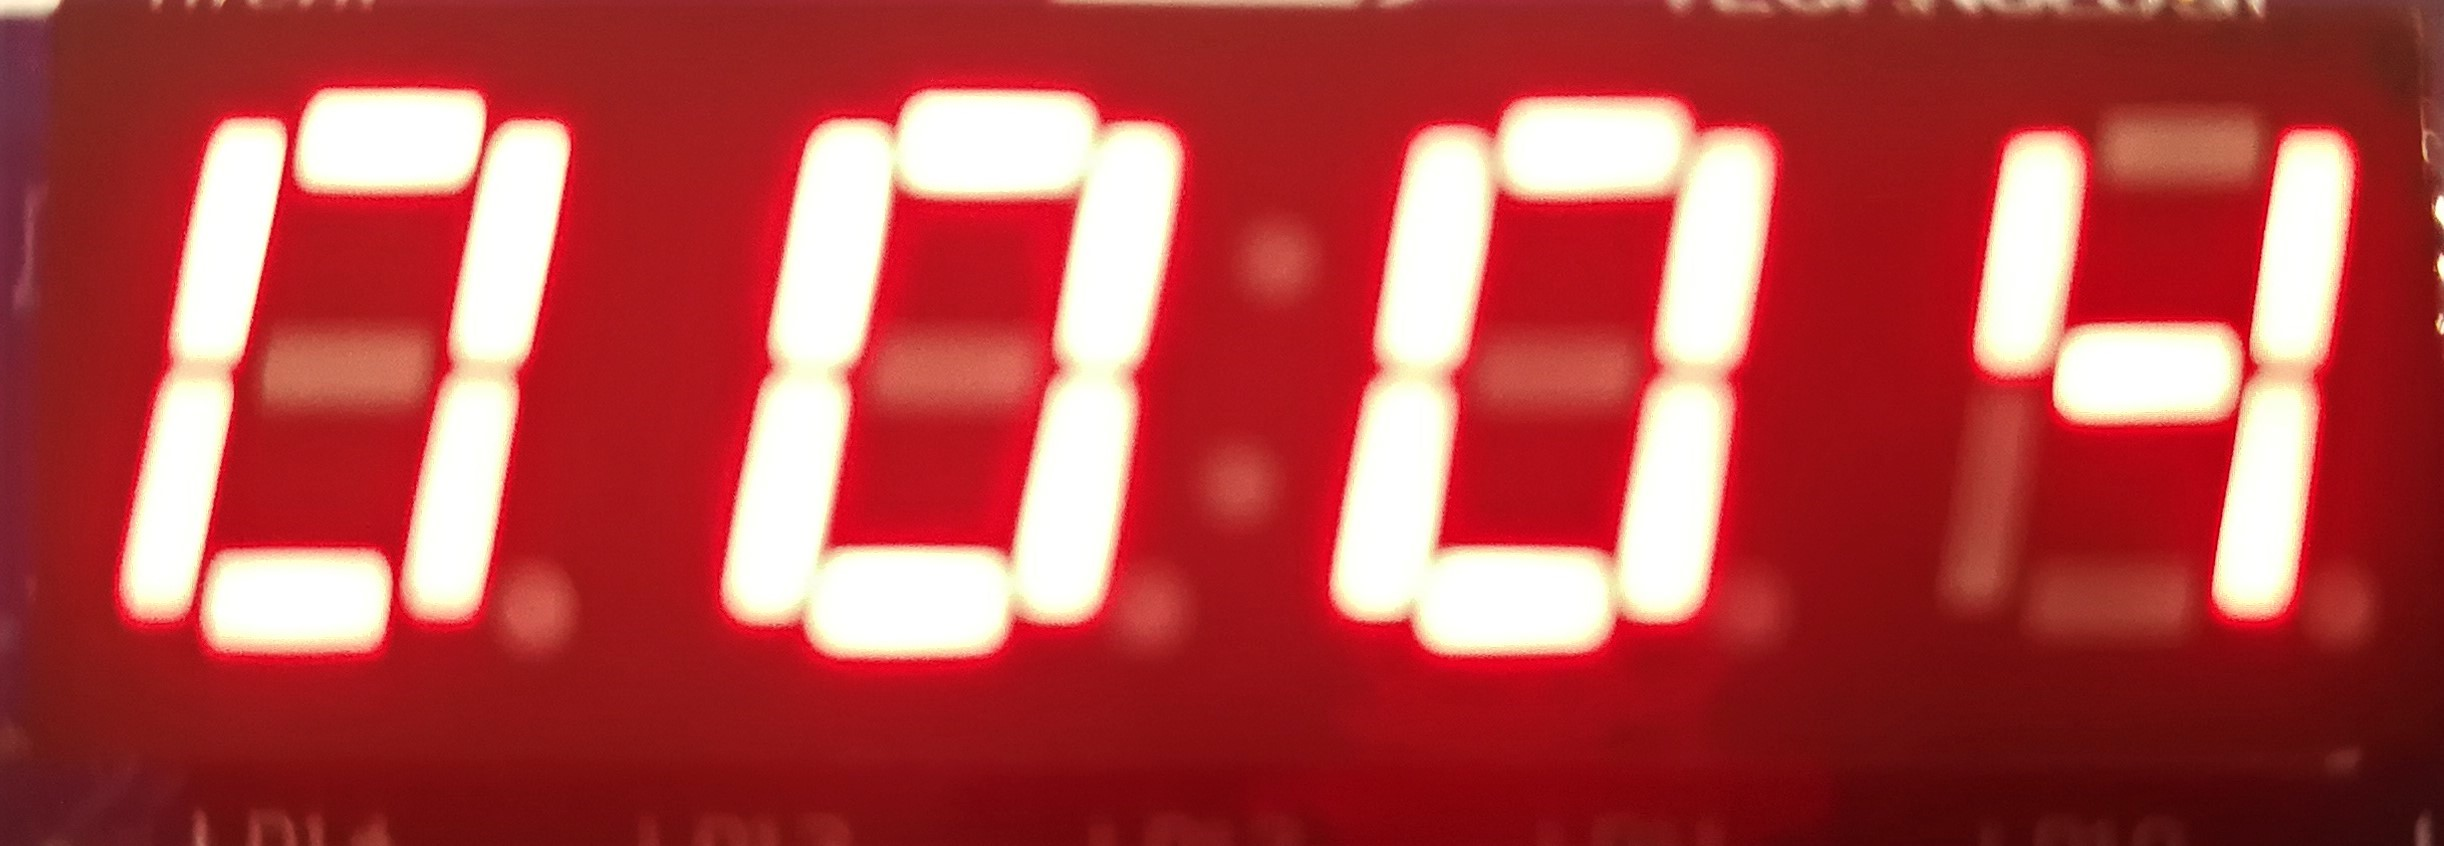
\includegraphics[width=0.3\linewidth]{fig/Implementation/0x00_00.jpg}&
    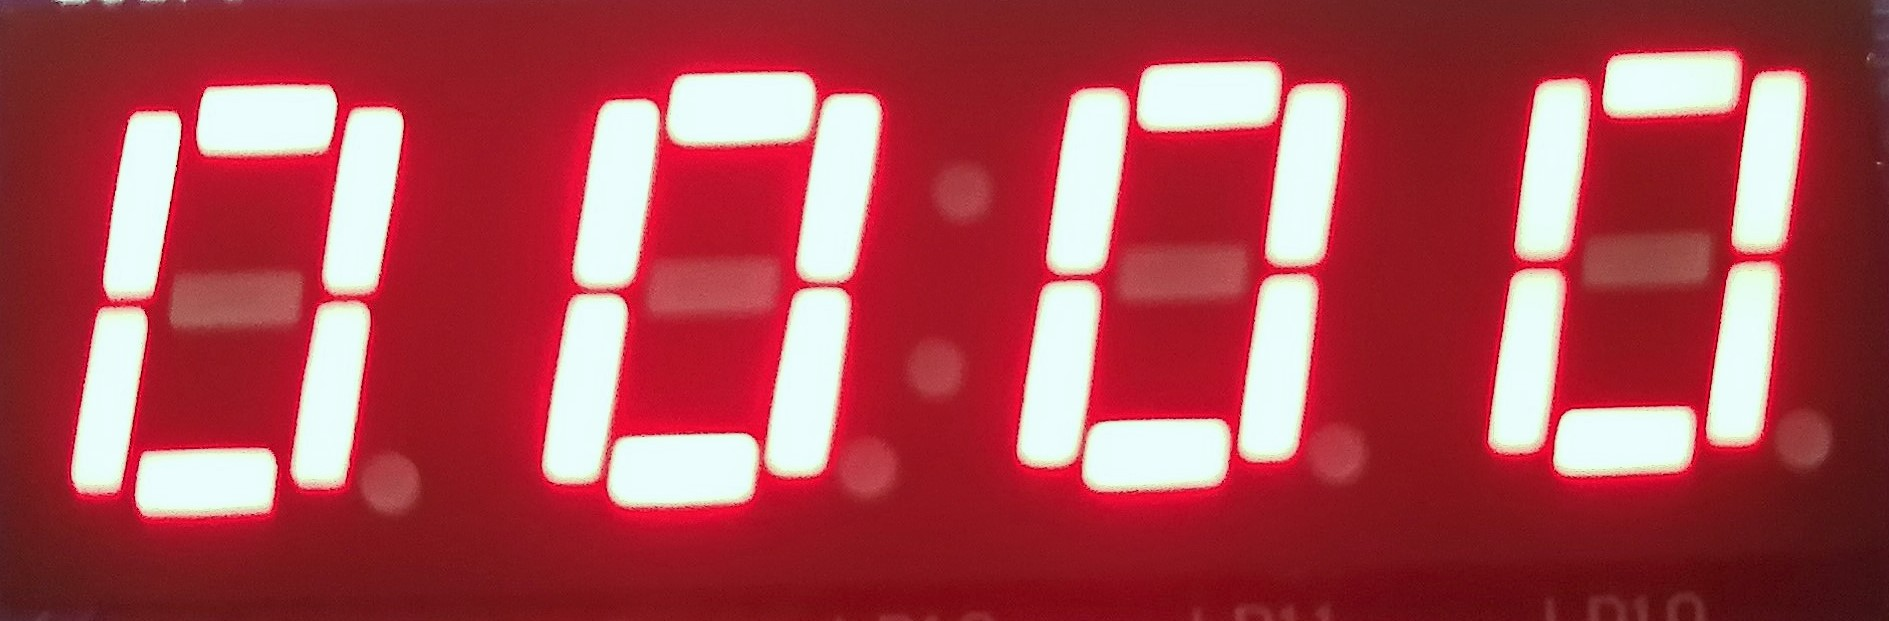
\includegraphics[width=0.3\linewidth]{fig/Implementation/0x00_01.jpg}\\
    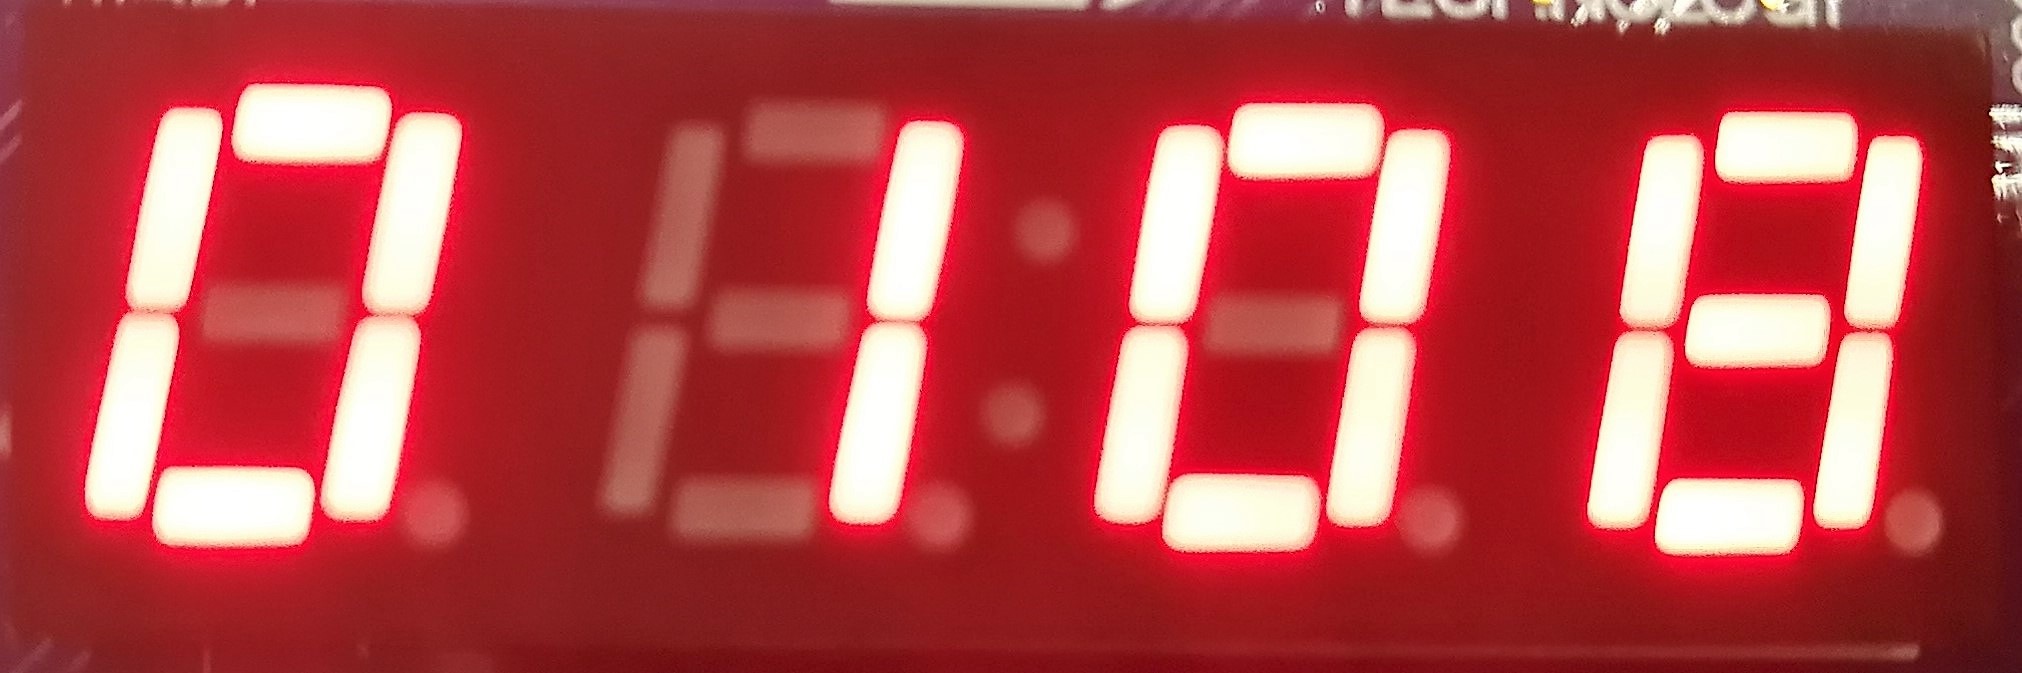
\includegraphics[width=0.3\linewidth]{fig/Implementation/0x00_10.jpg}&
    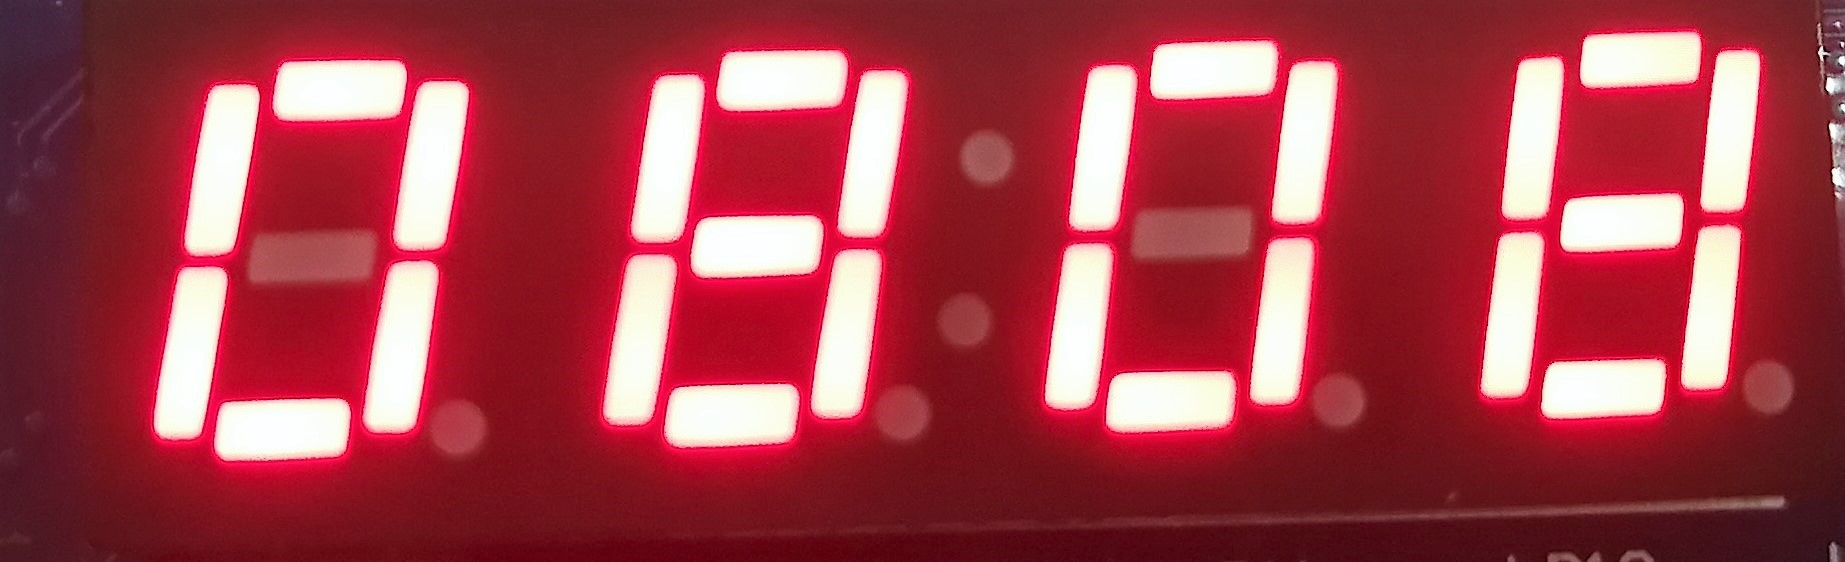
\includegraphics[width=0.3\linewidth]{fig/Implementation/0x00_11.jpg}
    \end{tabular}
    \caption{0x00结果}
    \end{figure}
    \item 0x0C: \verb'sub $5, $3, $2'
    \begin{figure}[H]
    \centering
    \begin{tabular}{cc}
    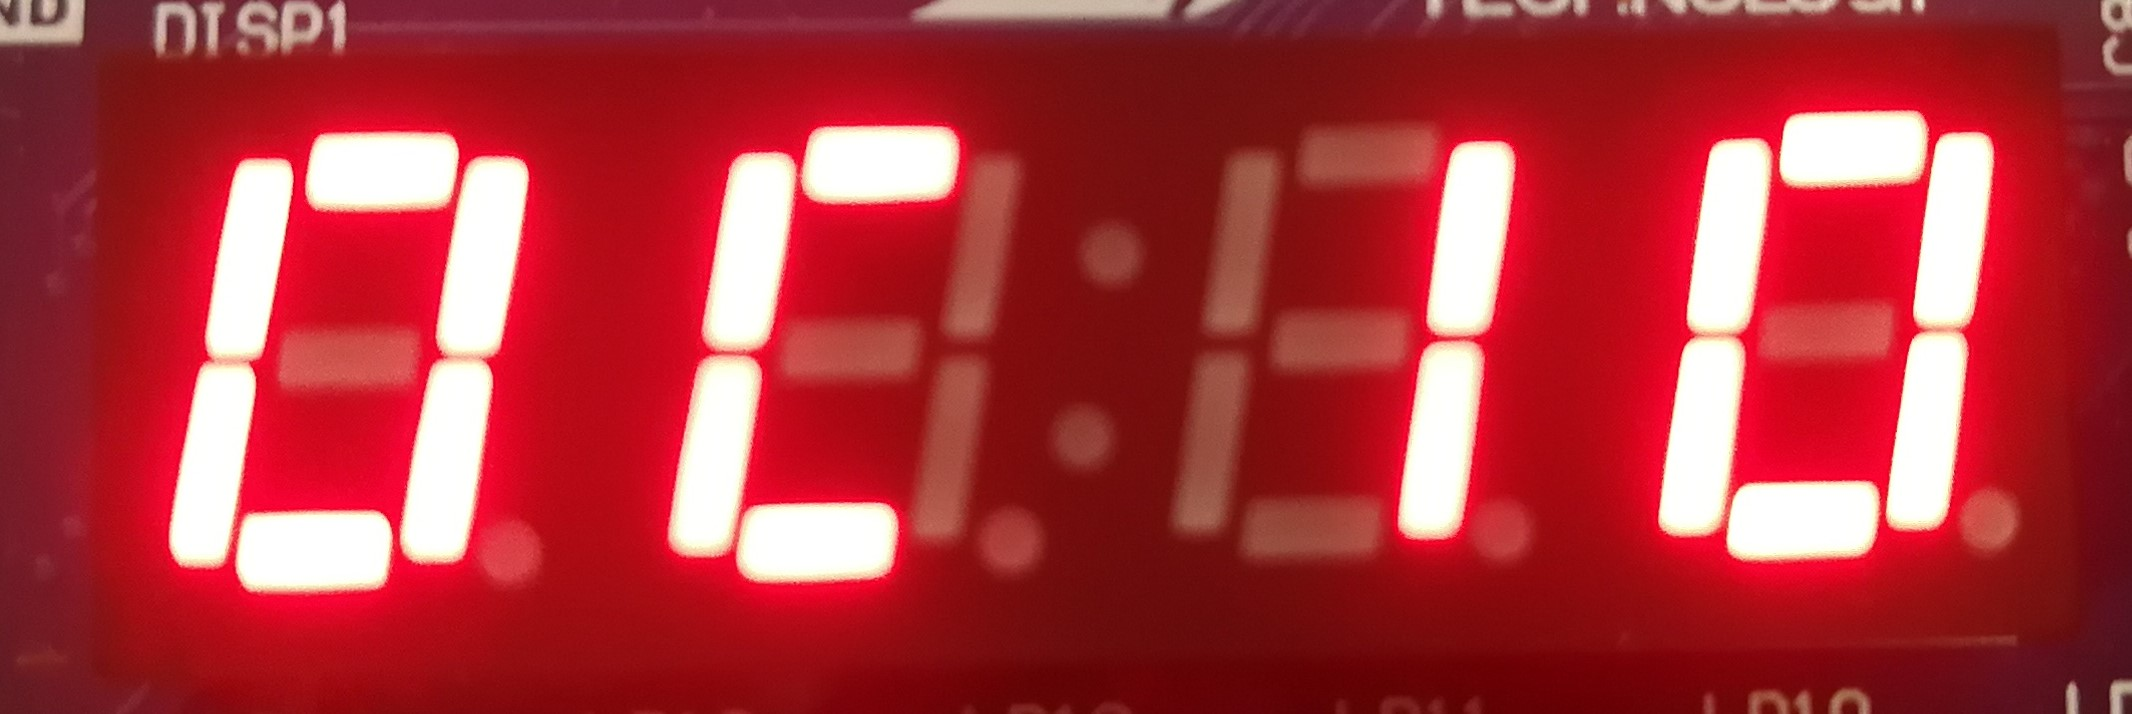
\includegraphics[width=0.3\linewidth]{fig/Implementation/0x0c_00.jpg}&
    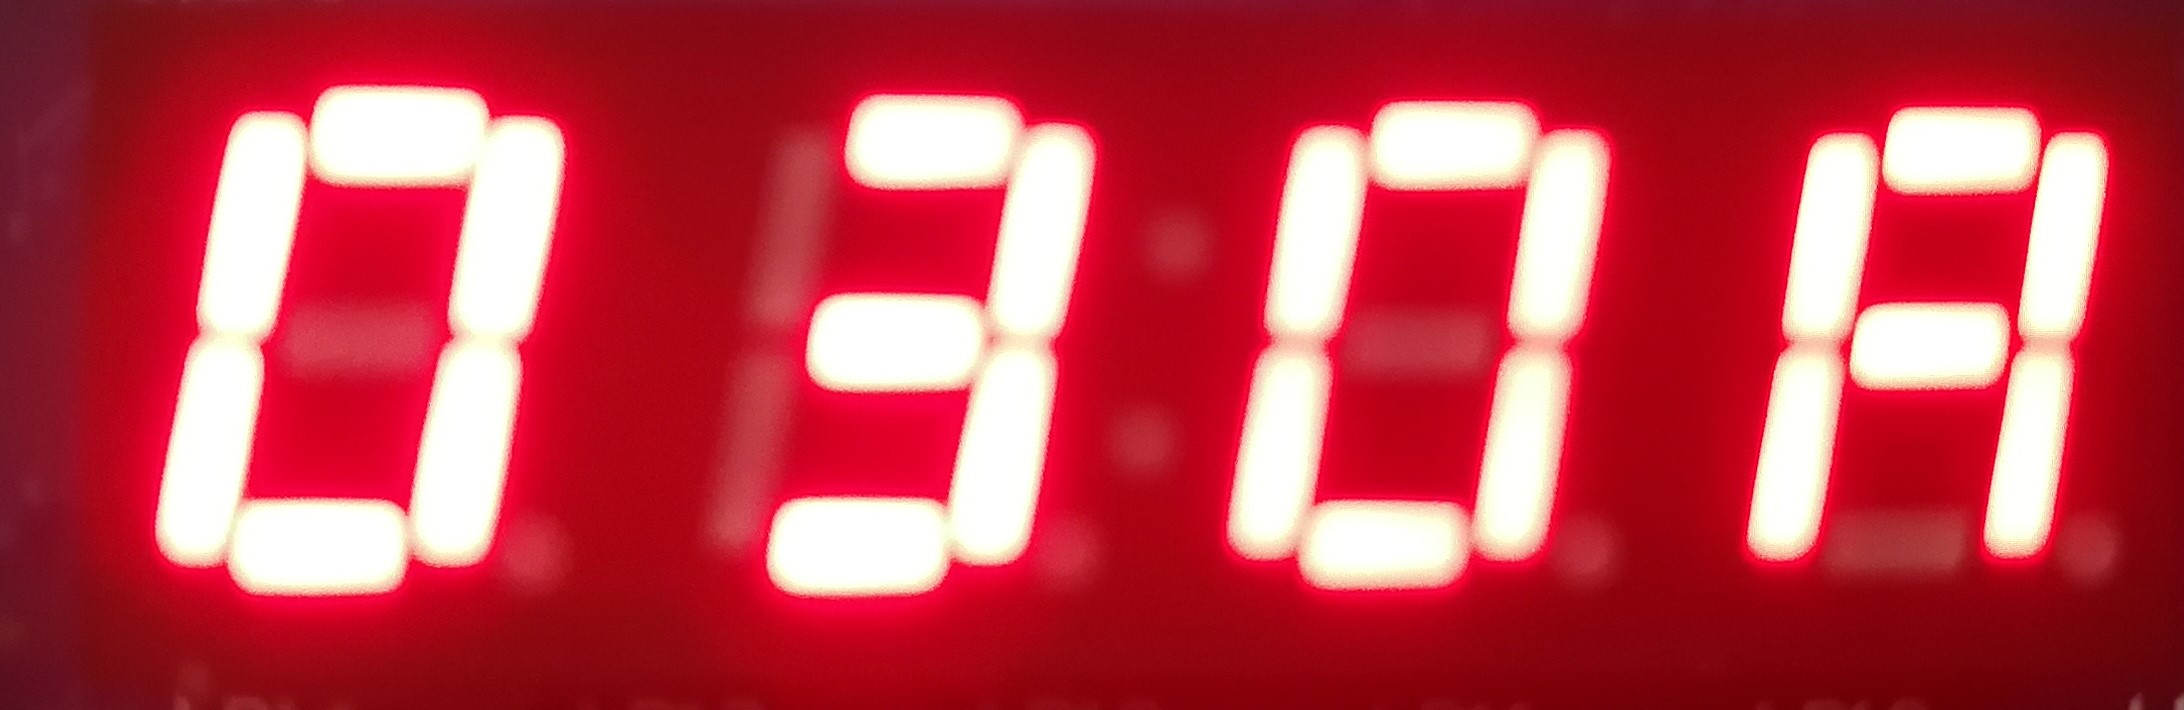
\includegraphics[width=0.3\linewidth]{fig/Implementation/0x0c_01.jpg}\\
    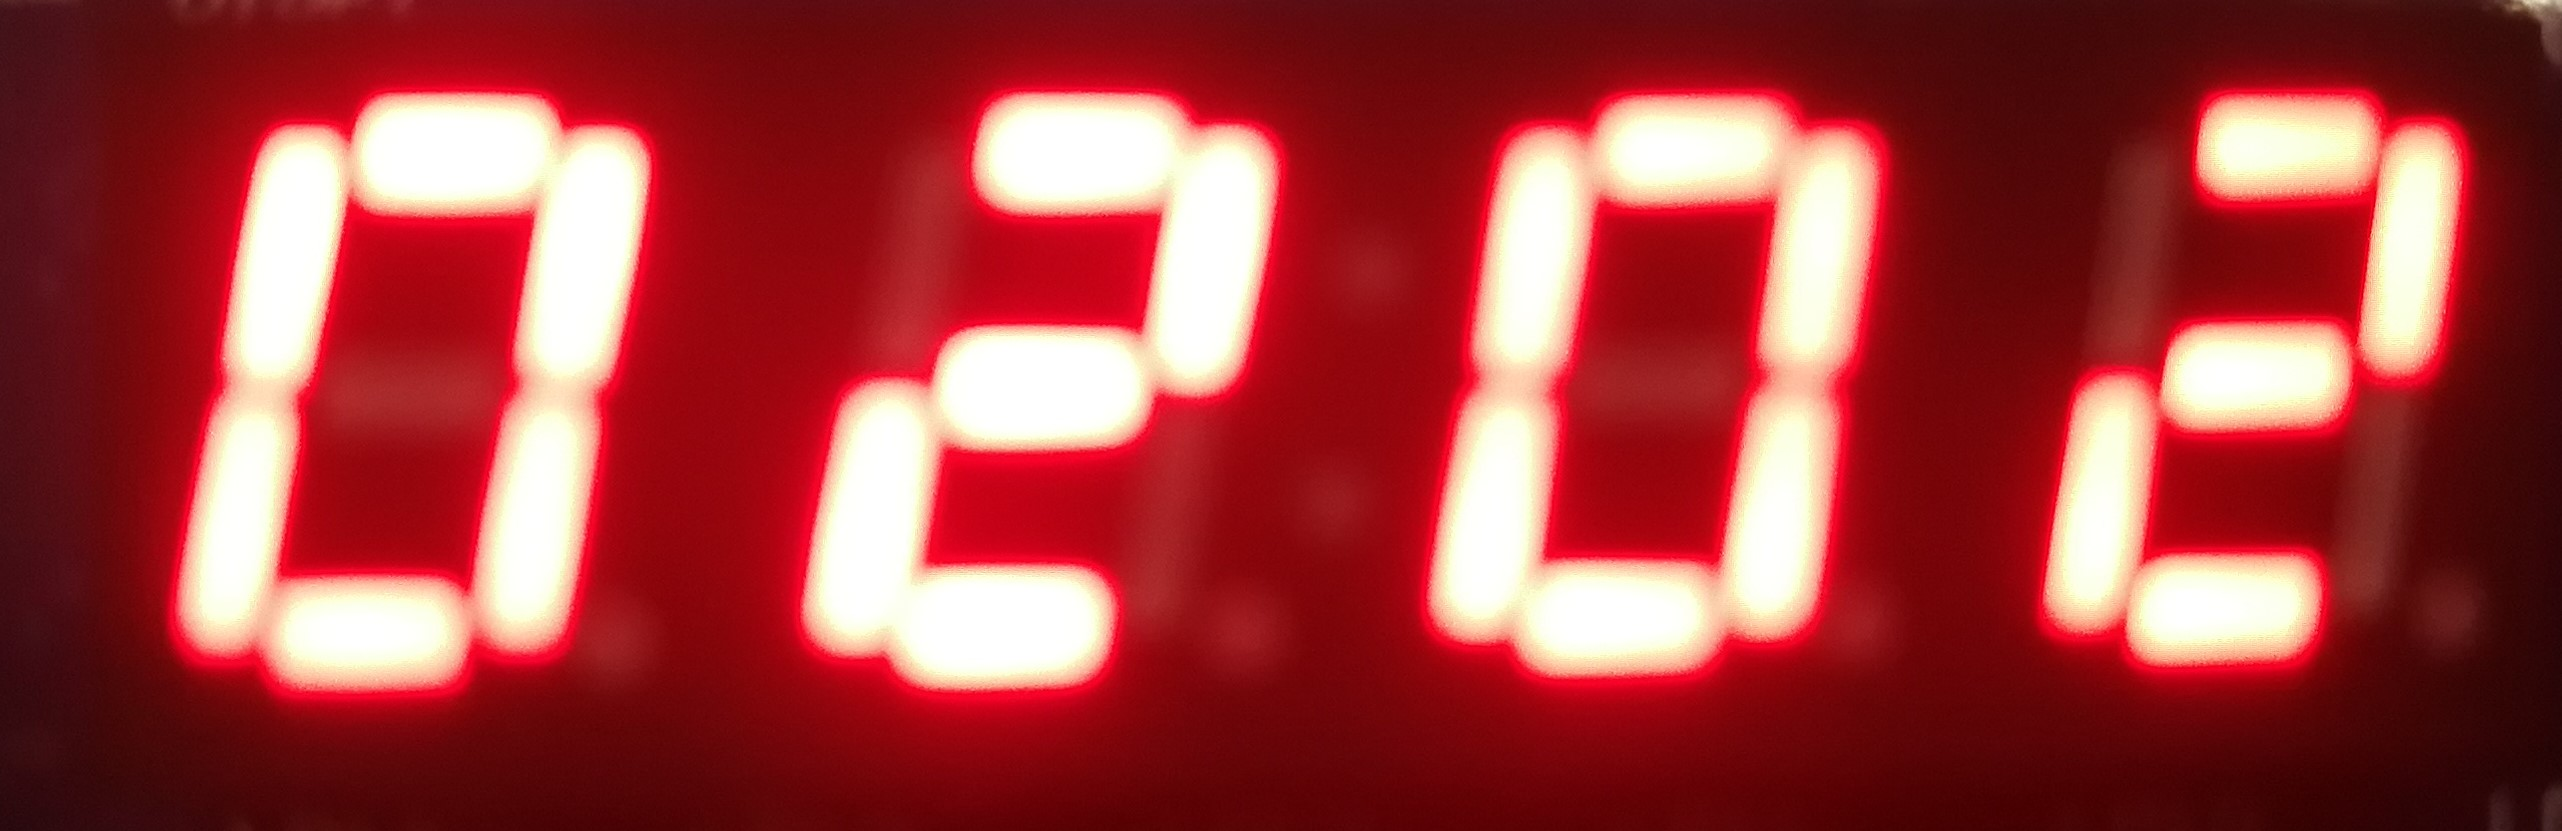
\includegraphics[width=0.3\linewidth]{fig/Implementation/0x0c_10.jpg}&
    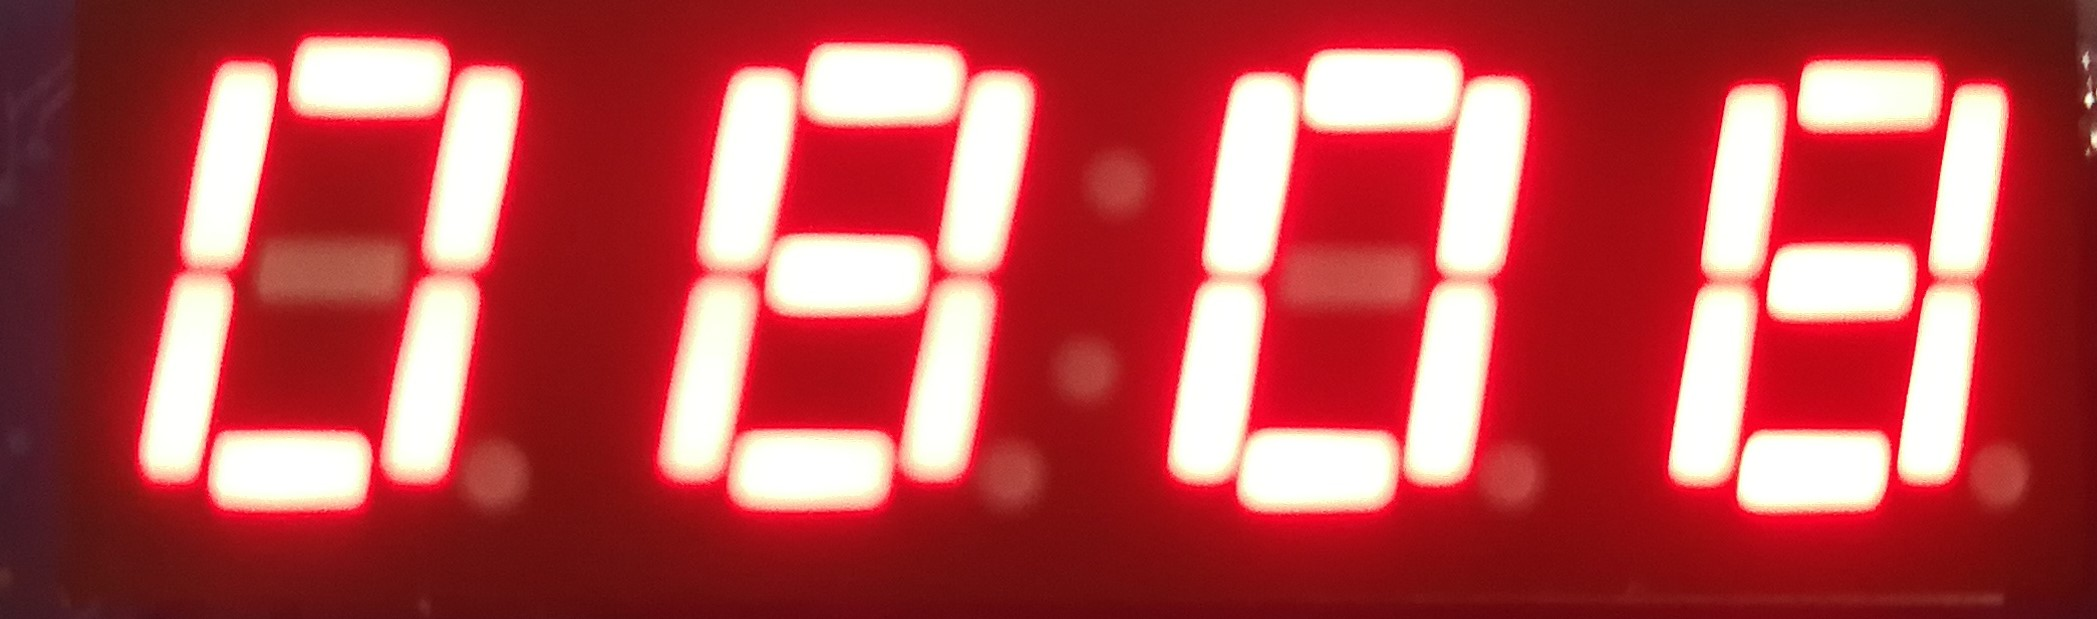
\includegraphics[width=0.3\linewidth]{fig/Implementation/0x0c_11.jpg}
    \end{tabular}
    \caption{0x0C结果}
    \end{figure}
    \item 0x14: \verb'or $8, $4, $2'
    \begin{figure}[H]
    \centering
    \begin{tabular}{cc}
    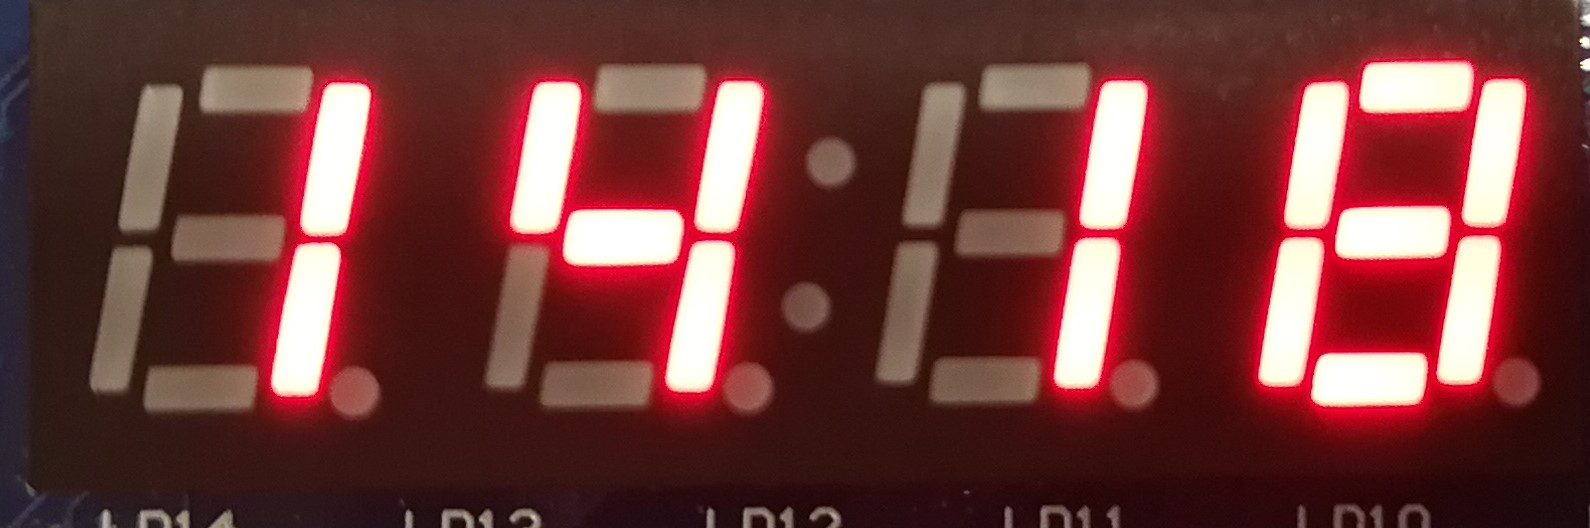
\includegraphics[width=0.3\linewidth]{fig/Implementation/0x14_00.jpg}&
    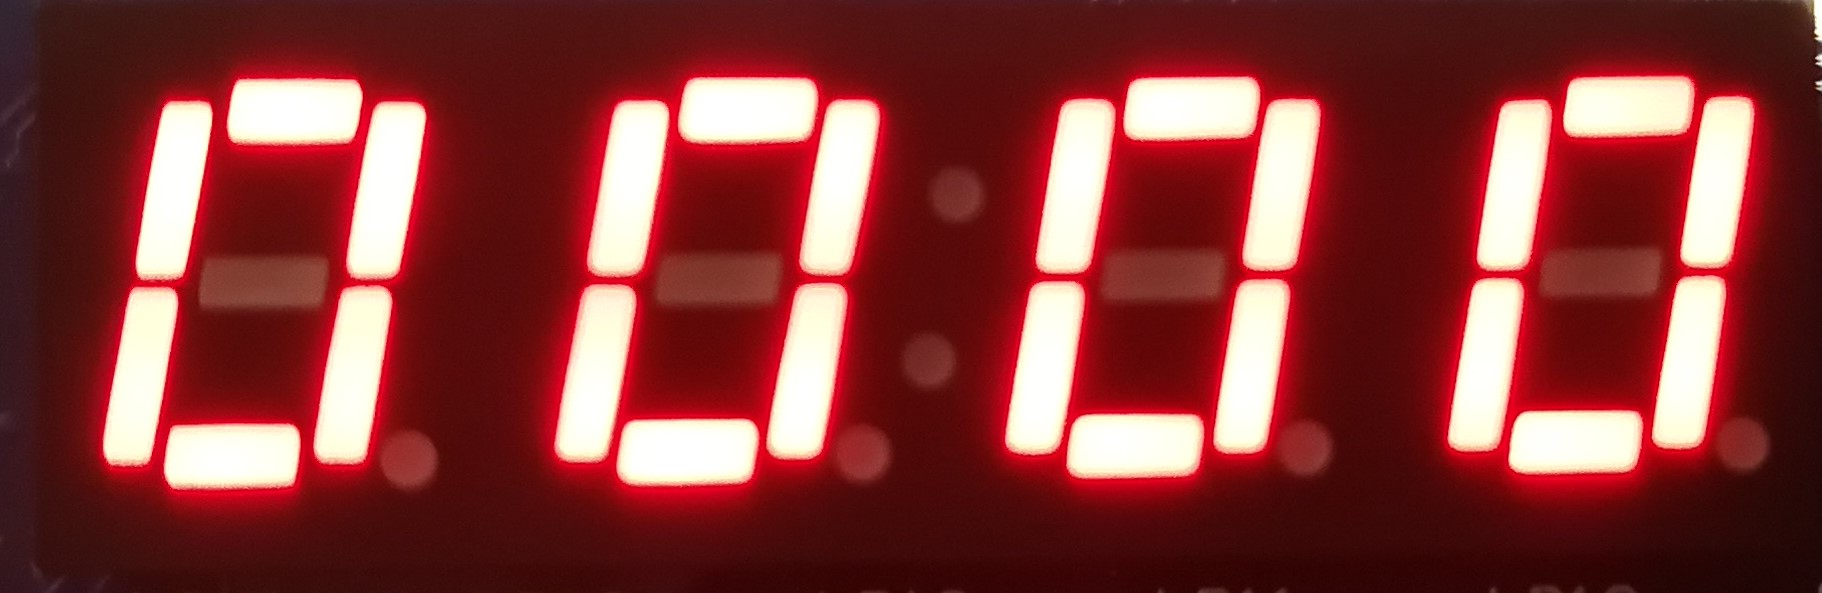
\includegraphics[width=0.3\linewidth]{fig/Implementation/0x14_01.jpg}\\
    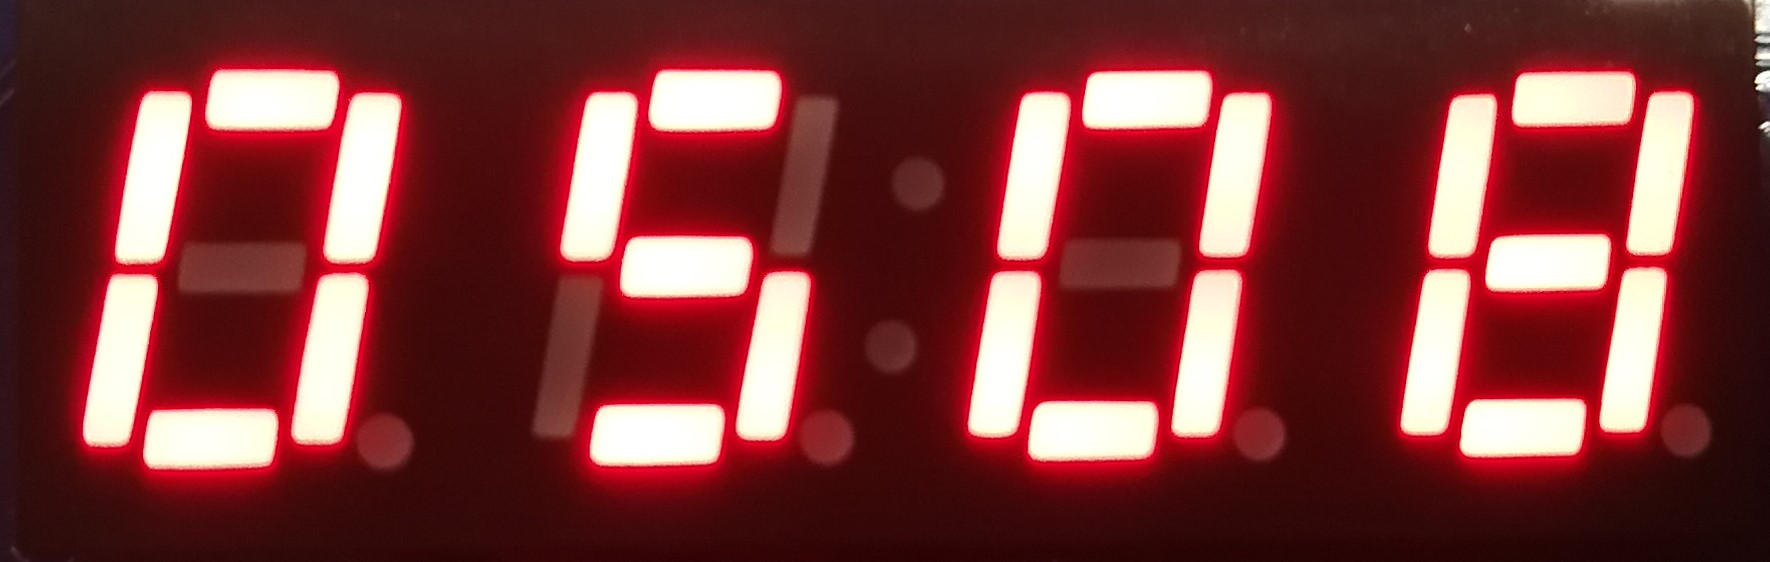
\includegraphics[width=0.3\linewidth]{fig/Implementation/0x14_10.jpg}&
    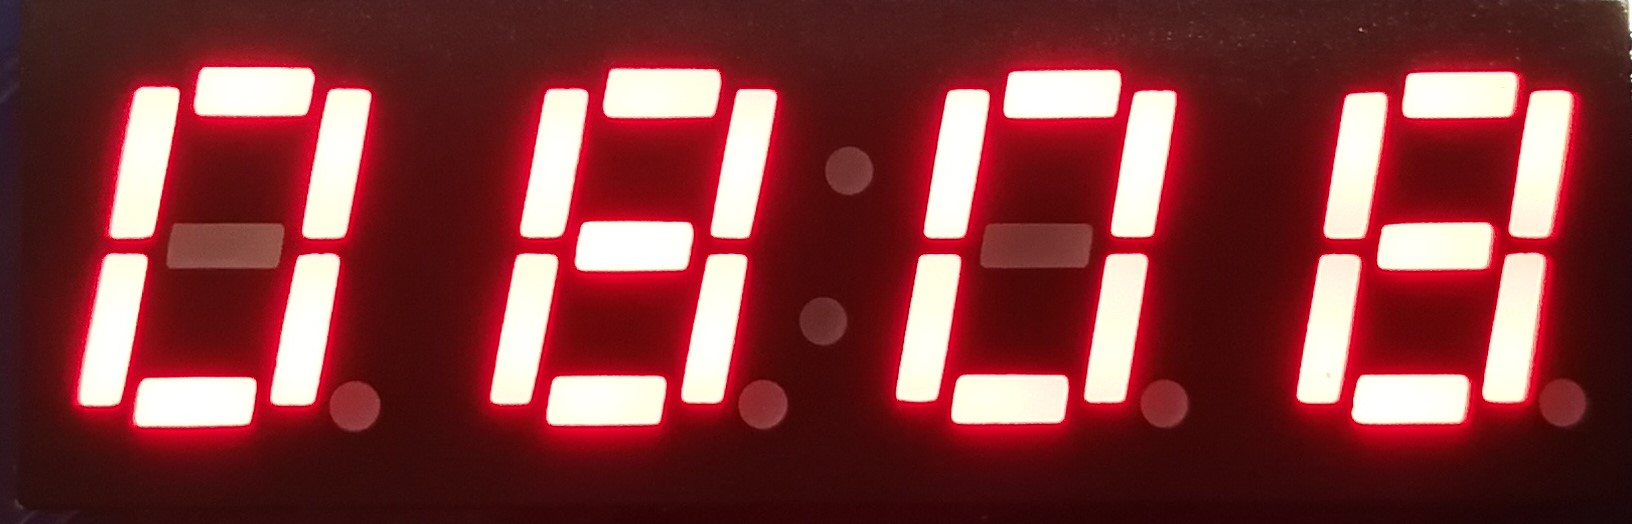
\includegraphics[width=0.3\linewidth]{fig/Implementation/0x14_11.jpg}
    \end{tabular}
    \caption{0x14结果}
    \end{figure}
    \item 0x18: \verb'sll $8, $8, 1'
    \begin{figure}[H]
    \centering
    \begin{tabular}{cc}
    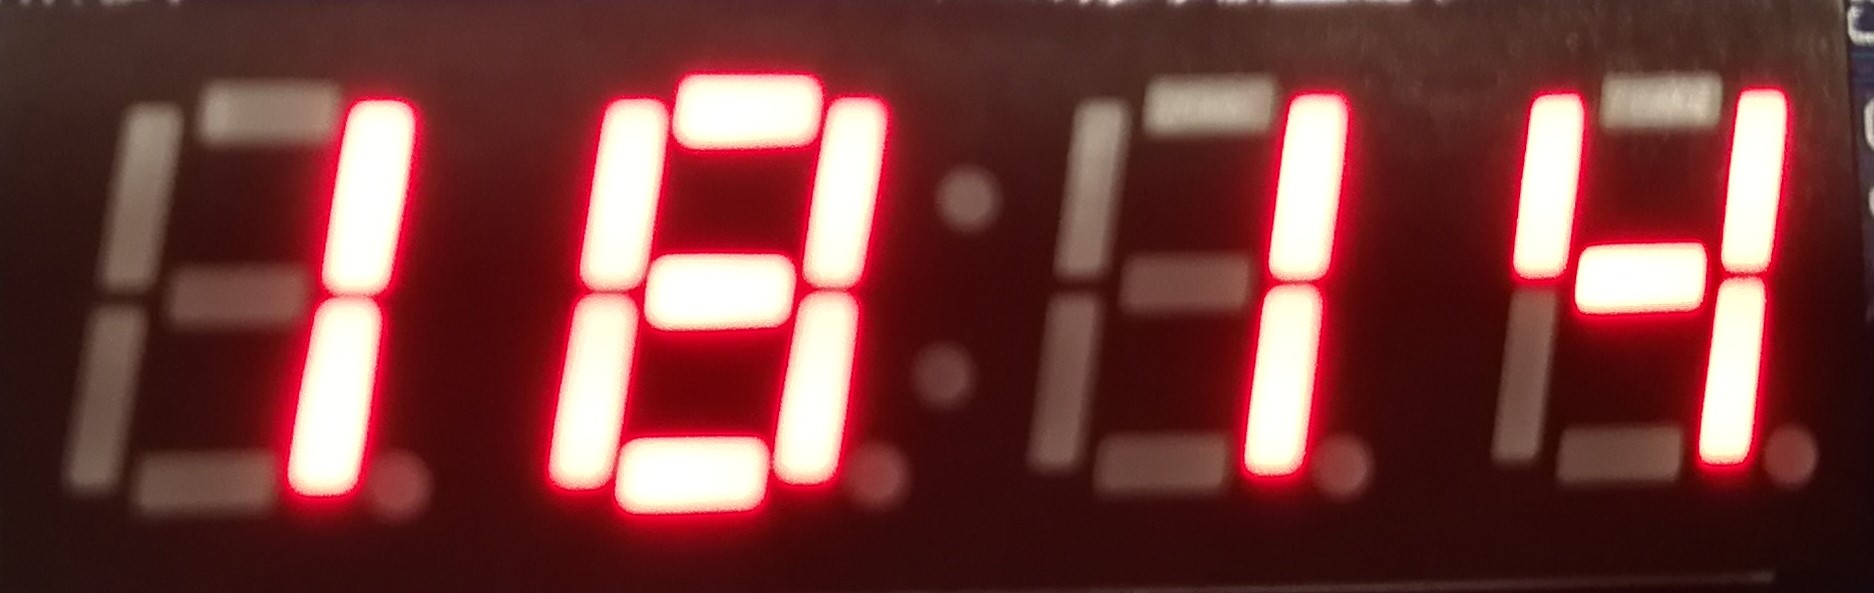
\includegraphics[width=0.3\linewidth]{fig/Implementation/0x18_00.jpg}&
    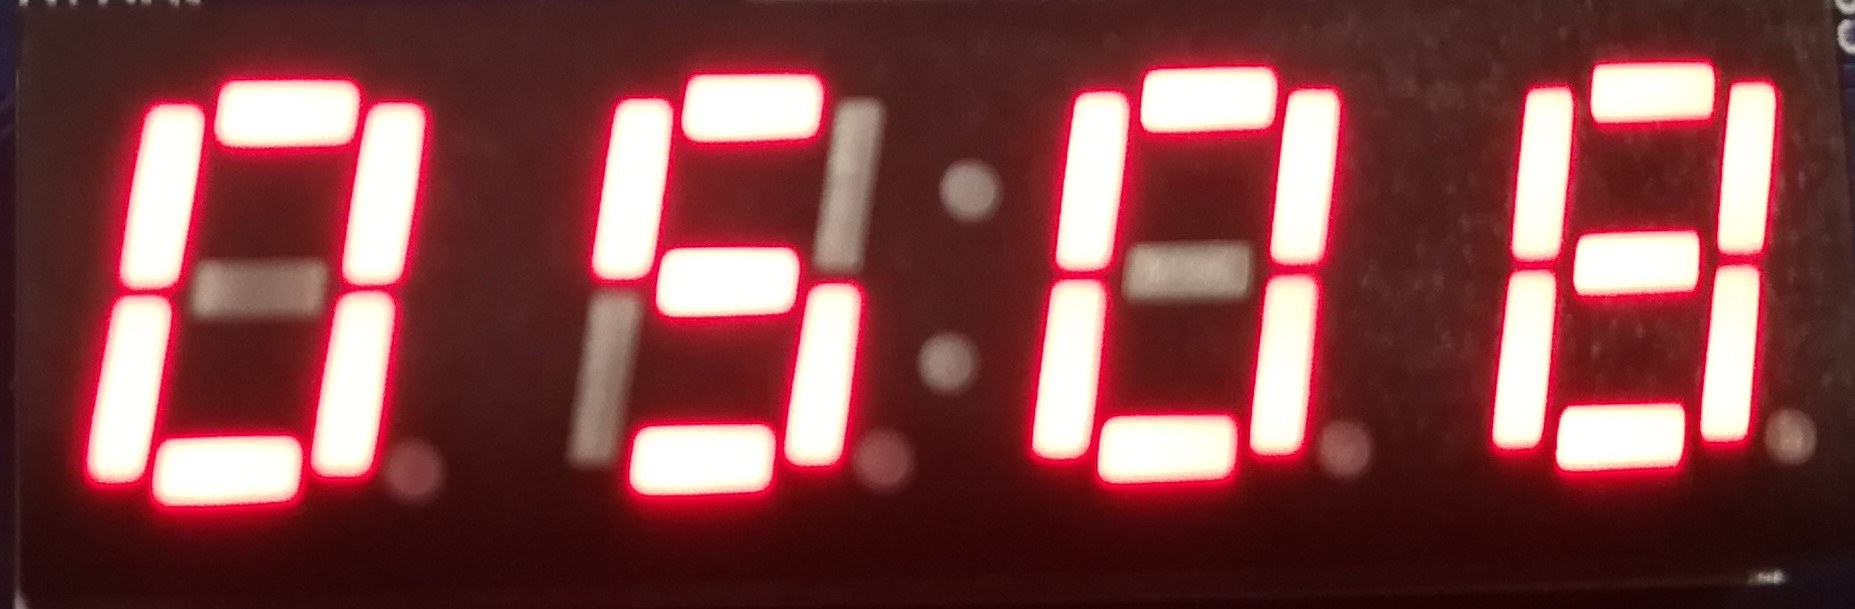
\includegraphics[width=0.3\linewidth]{fig/Implementation/0x18_01.jpg}\\
    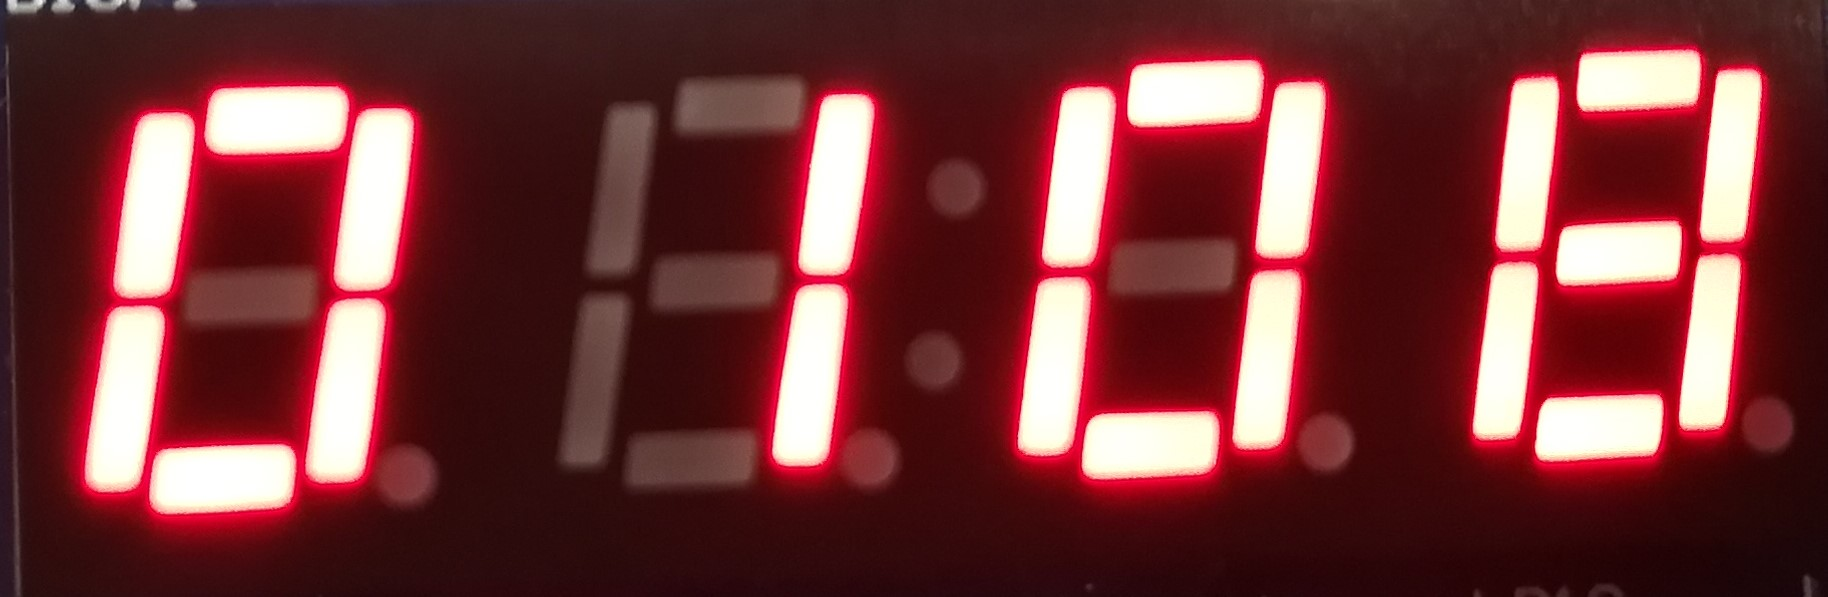
\includegraphics[width=0.3\linewidth]{fig/Implementation/0x18_10.jpg}&
    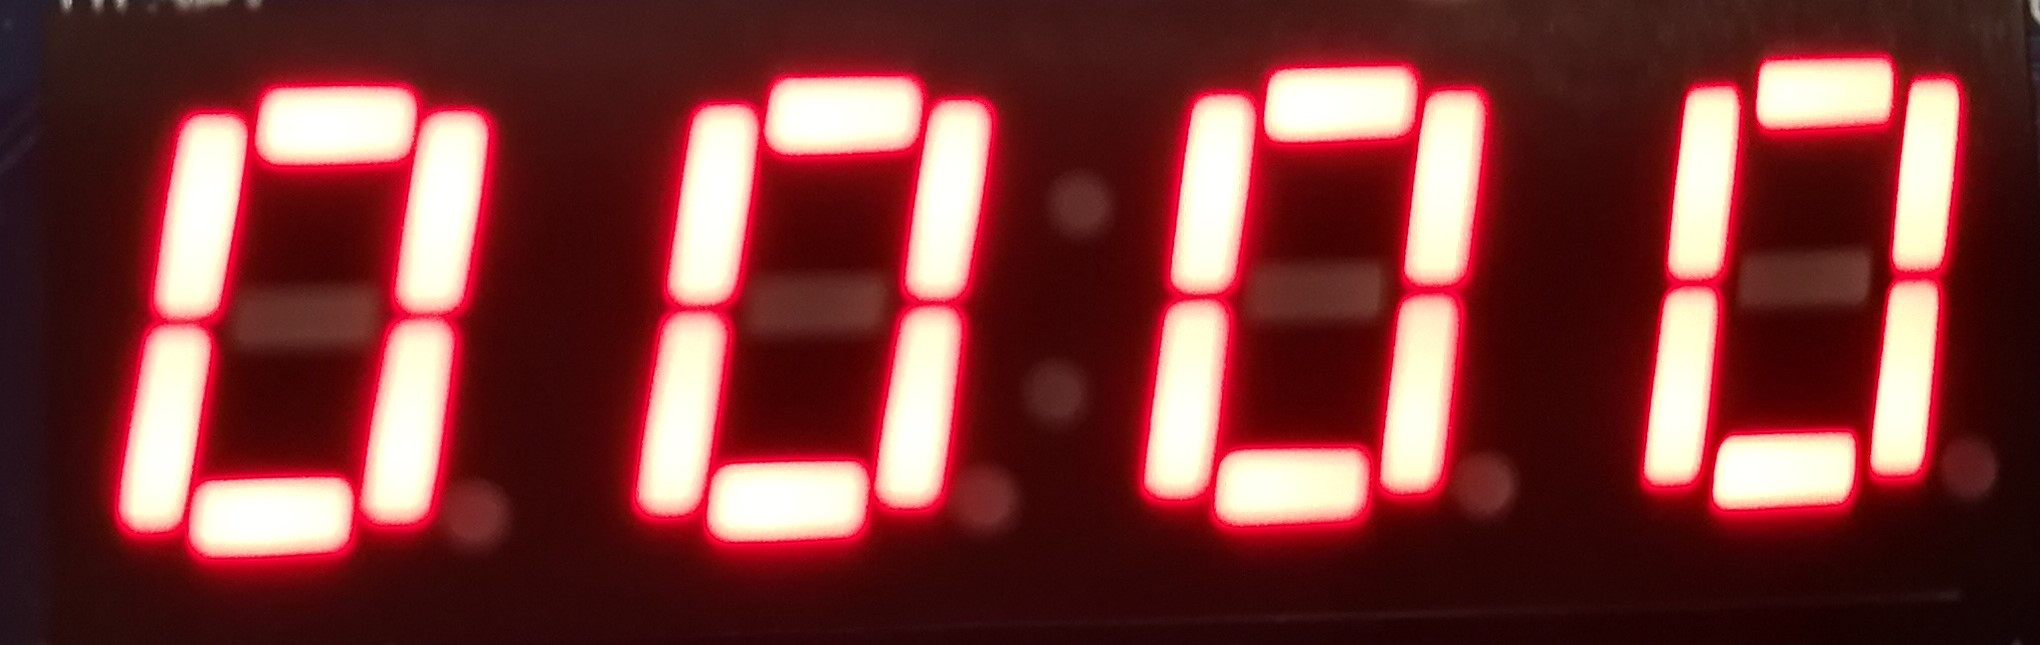
\includegraphics[width=0.3\linewidth]{fig/Implementation/0x18_11.jpg}
    \end{tabular}
    \caption{0x18结果}
    \end{figure}
    \item 0x1C: \verb'bne $8, $1, -2'
    \begin{figure}[H]
    \centering
    \begin{tabular}{cc}
    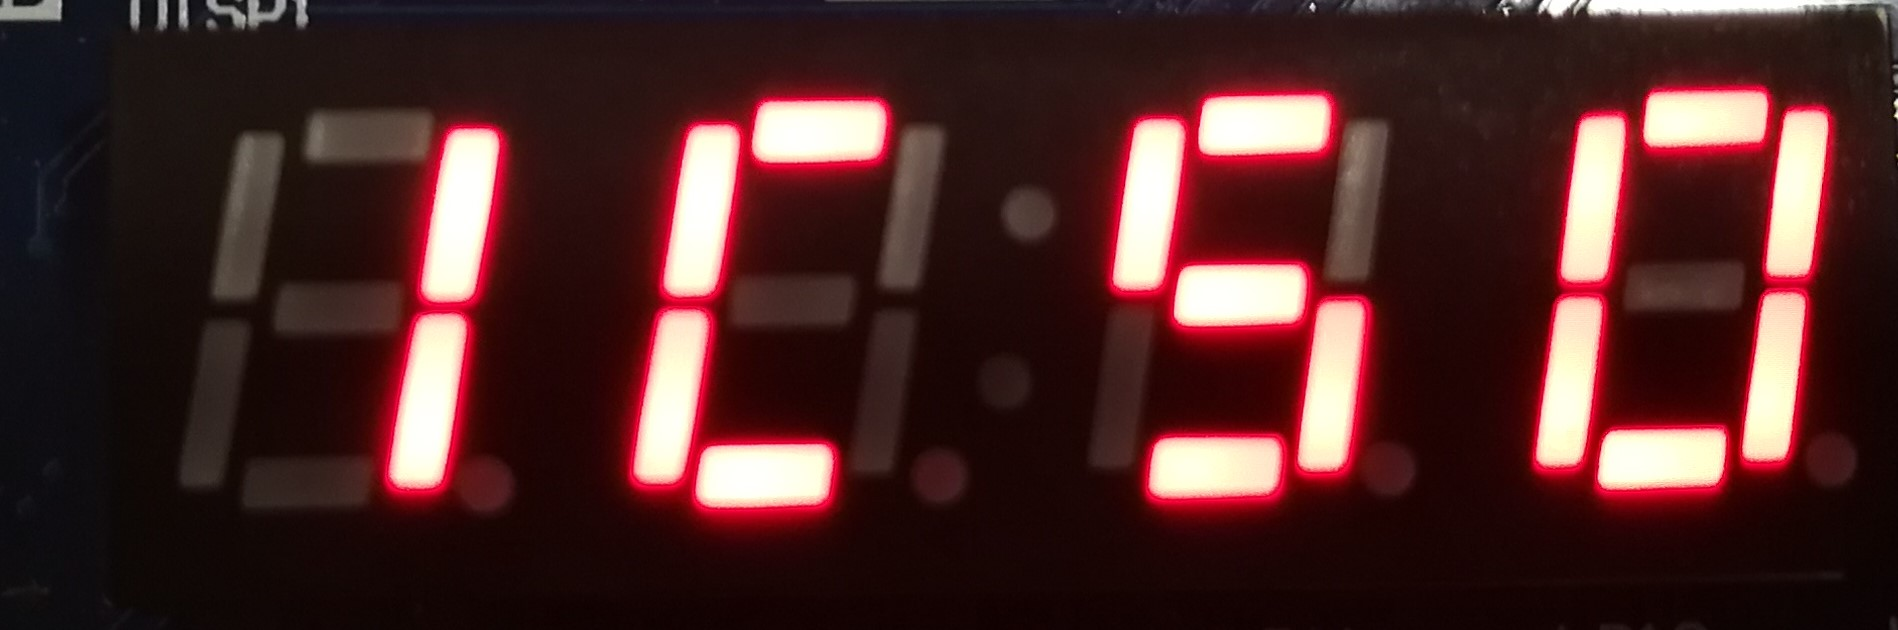
\includegraphics[width=0.3\linewidth]{fig/Implementation/0x1c_00.jpg}&
    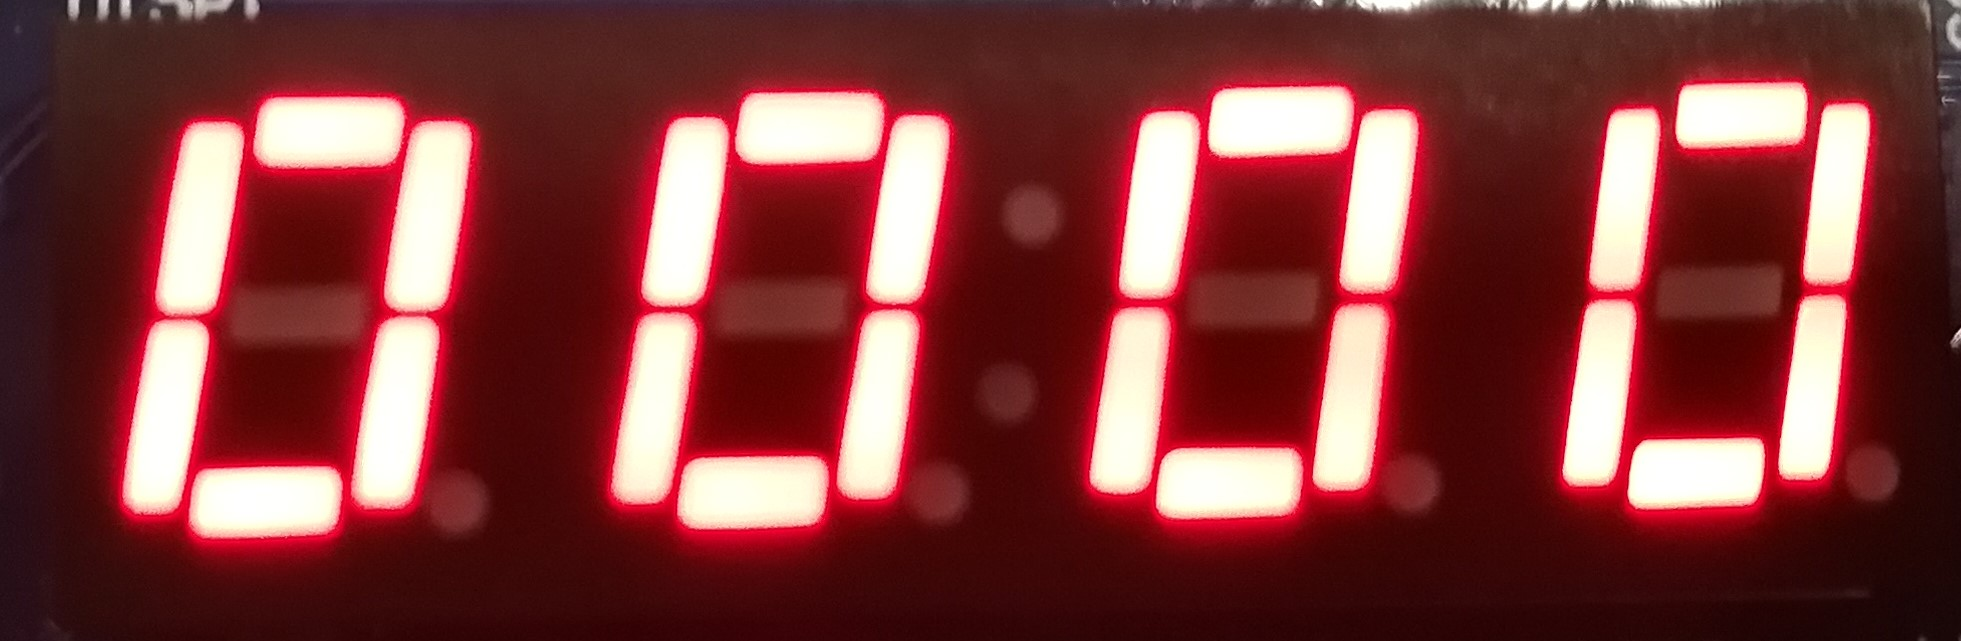
\includegraphics[width=0.3\linewidth]{fig/Implementation/0x1c_01.jpg}\\
    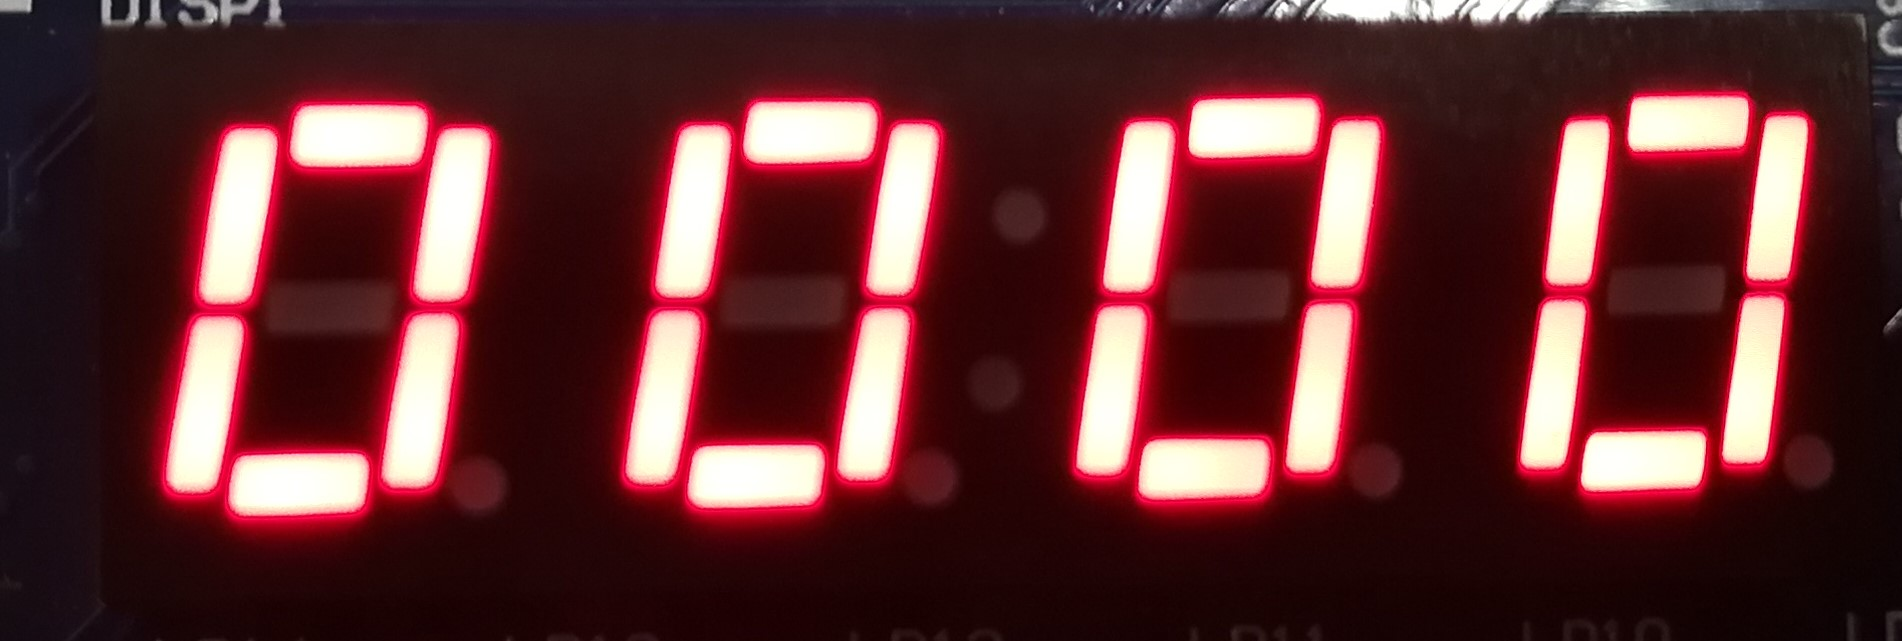
\includegraphics[width=0.3\linewidth]{fig/Implementation/0x1c_10.jpg}&
    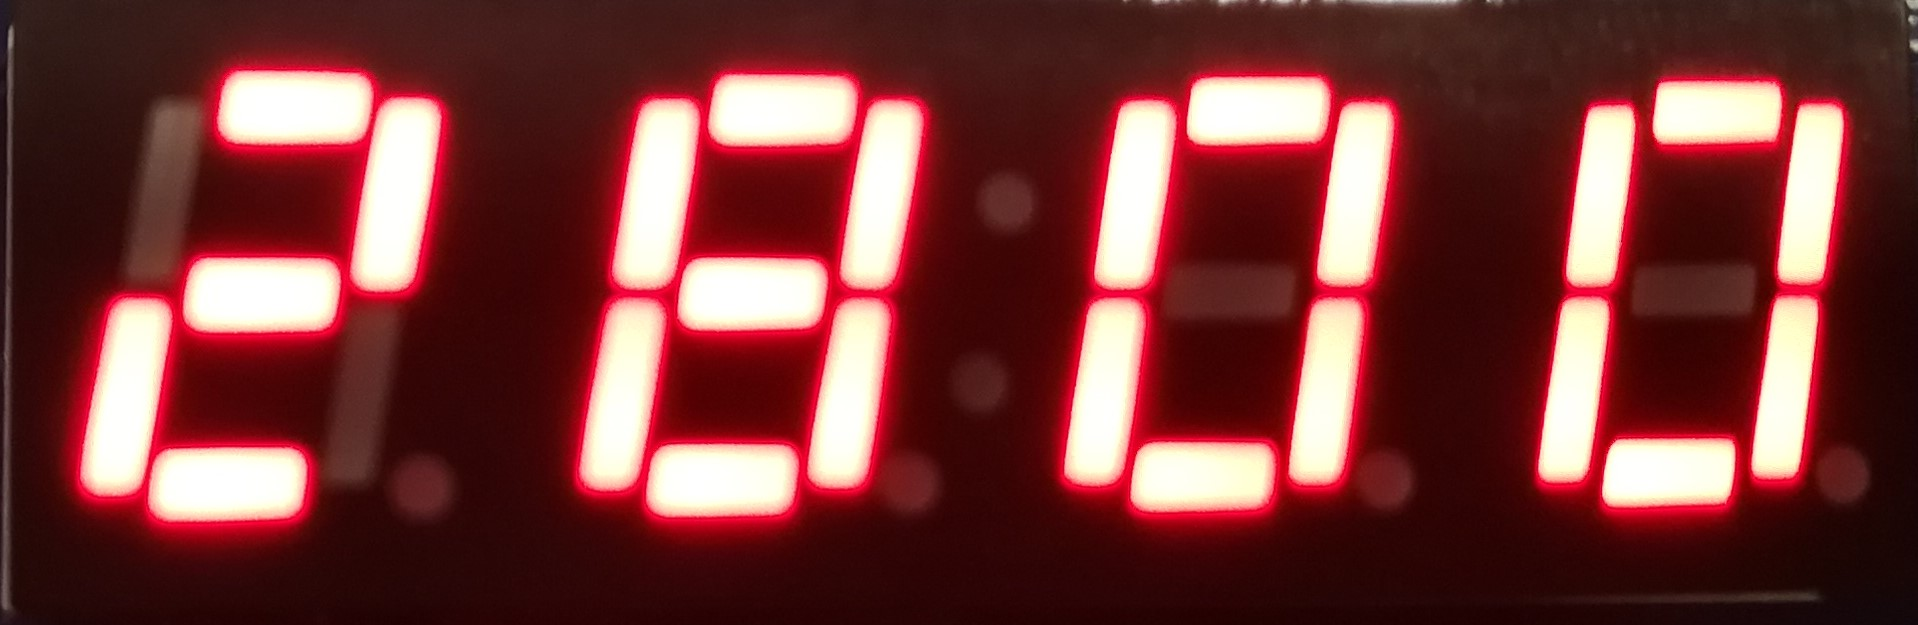
\includegraphics[width=0.3\linewidth]{fig/Implementation/0x1c_11.jpg}
    \end{tabular}
    \caption{0x1C结果}
    \end{figure}
    \item 0x30: \verb'sw $2, 4($1)'
    \begin{figure}[H]
    \centering
    \begin{tabular}{cc}
    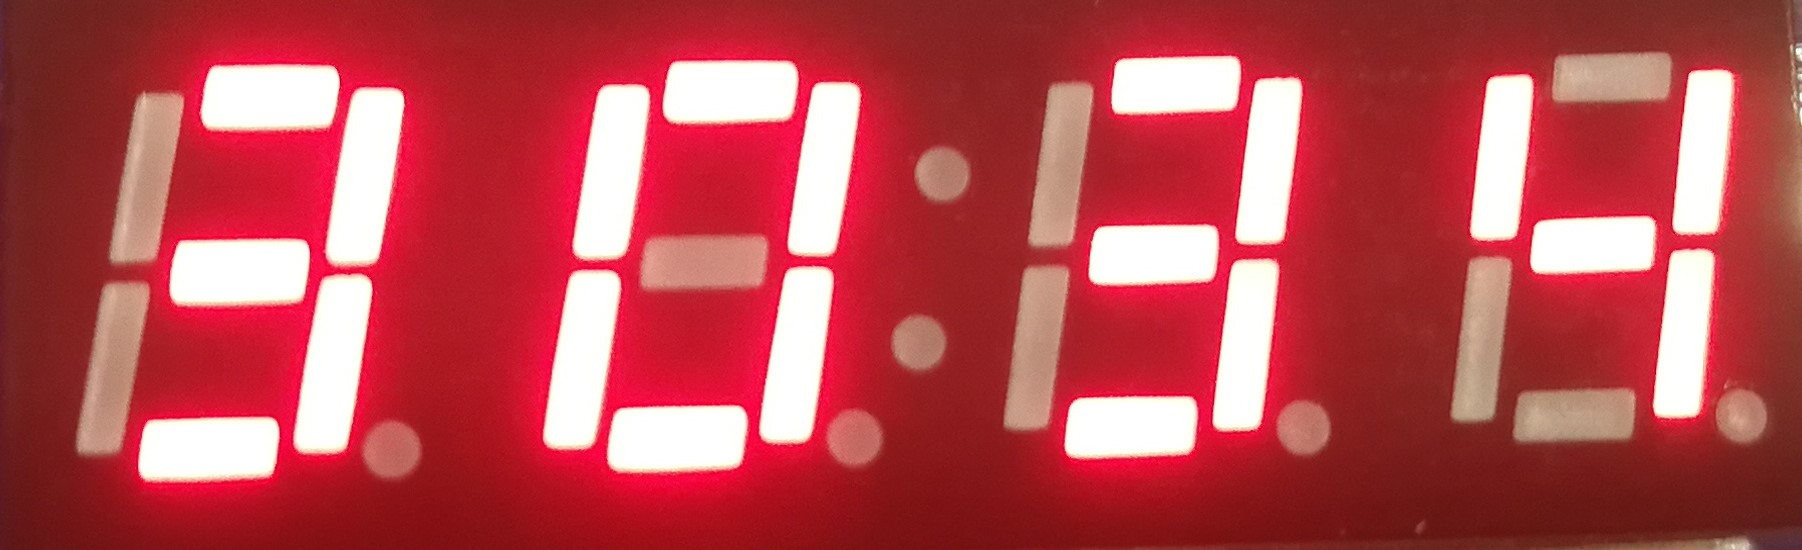
\includegraphics[width=0.3\linewidth]{fig/Implementation/0x30_00.jpg}&
    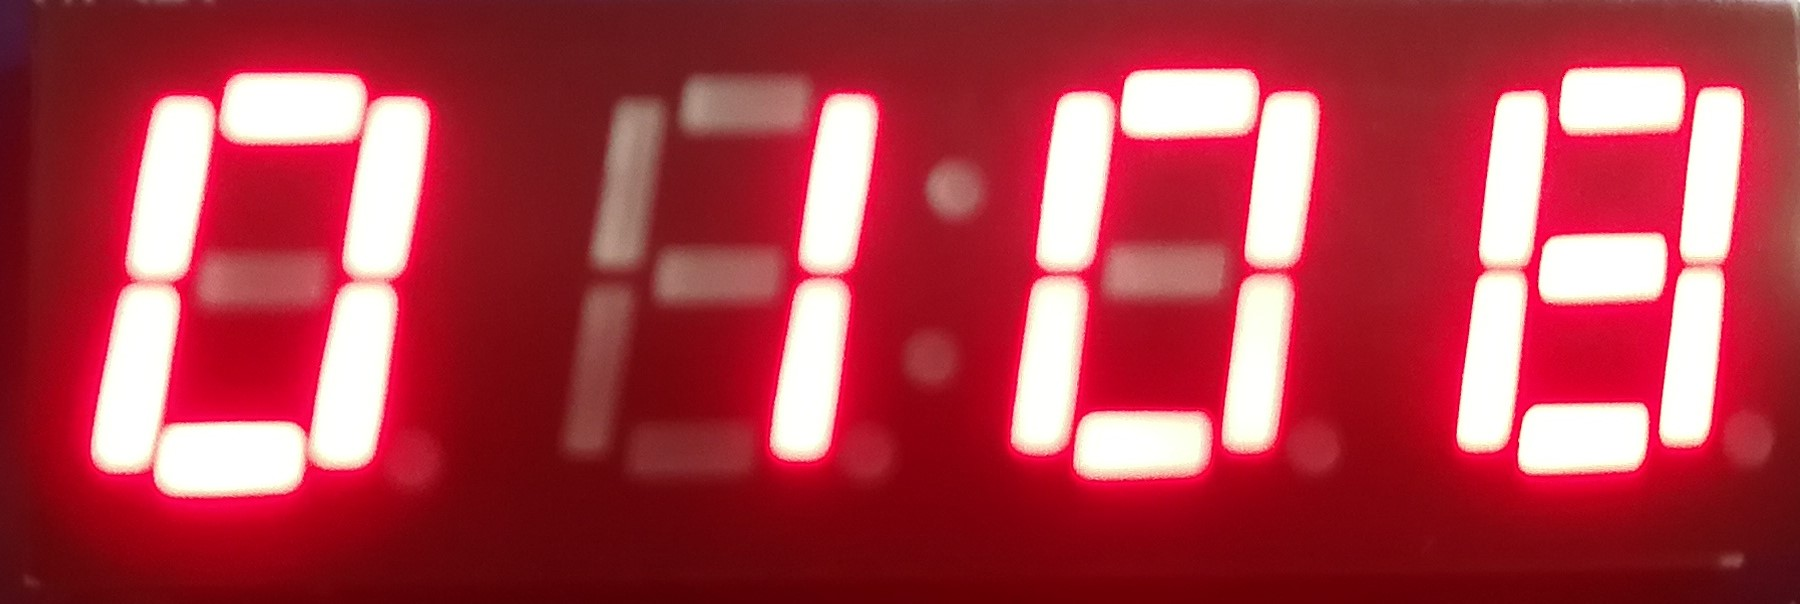
\includegraphics[width=0.3\linewidth]{fig/Implementation/0x30_01.jpg}\\
    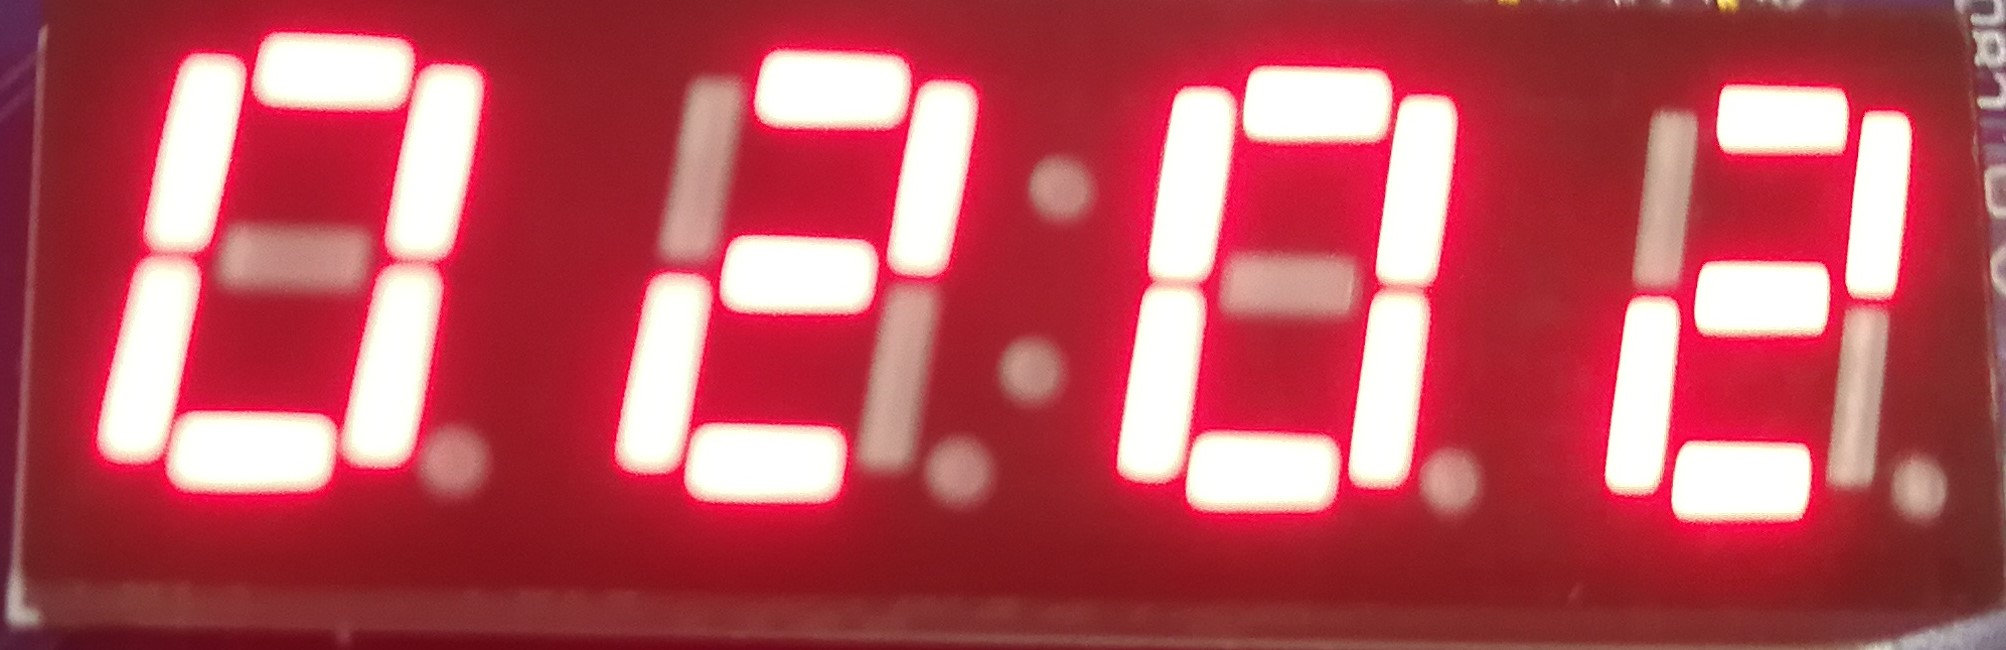
\includegraphics[width=0.3\linewidth]{fig/Implementation/0x30_10.jpg}&
    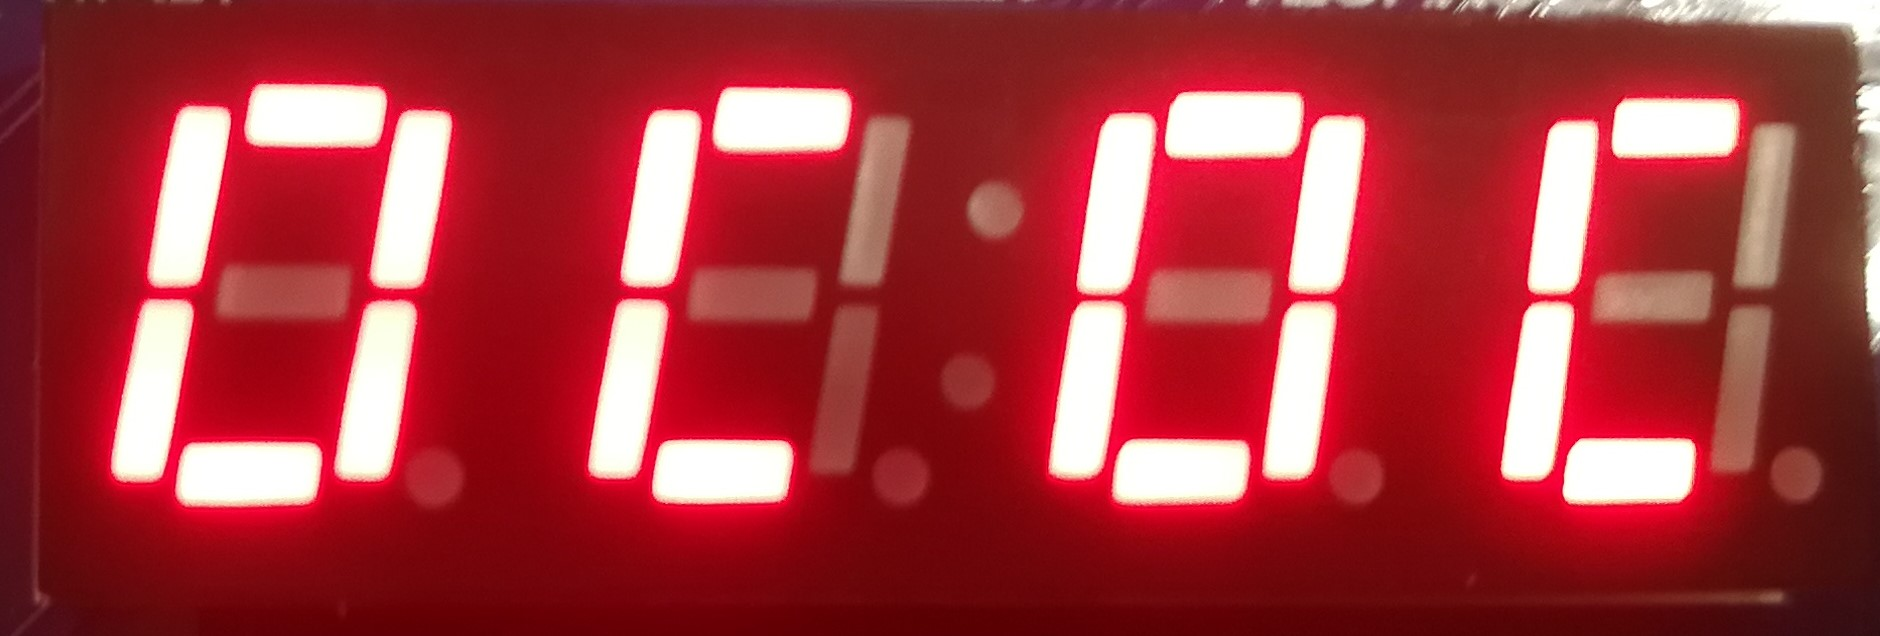
\includegraphics[width=0.3\linewidth]{fig/Implementation/0x30_11.jpg}
    \end{tabular}
    \caption{0x30结果}
    \end{figure}
    \item 0x34: \verb'lw $9, 4($1)'
    \begin{figure}[H]
    \centering
    \begin{tabular}{cc}
    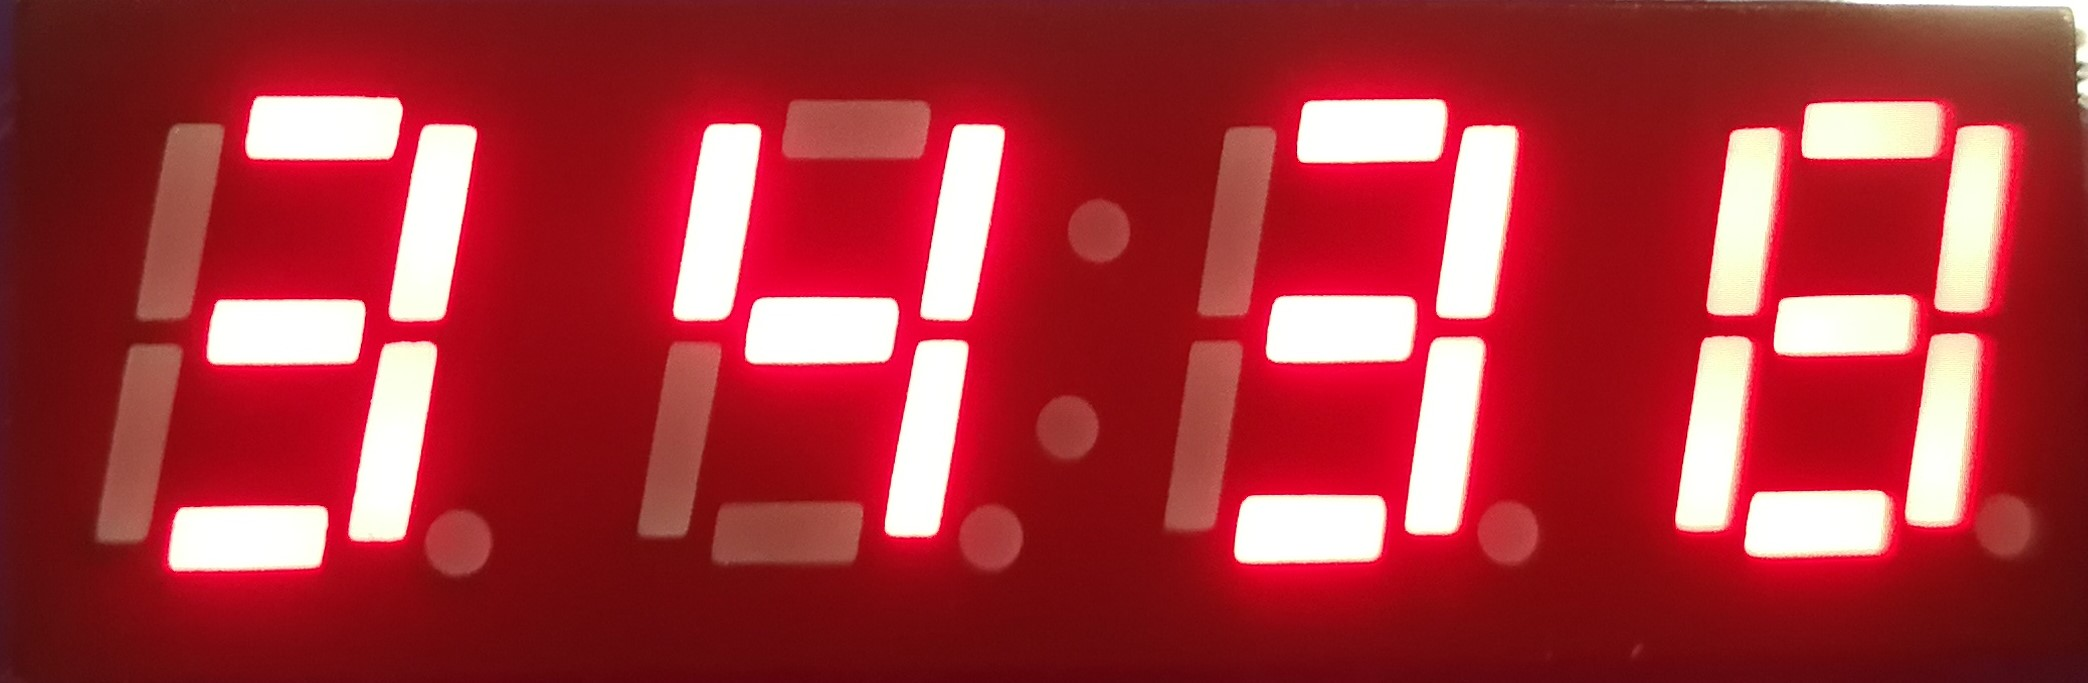
\includegraphics[width=0.3\linewidth]{fig/Implementation/0x34_00.jpg}&
    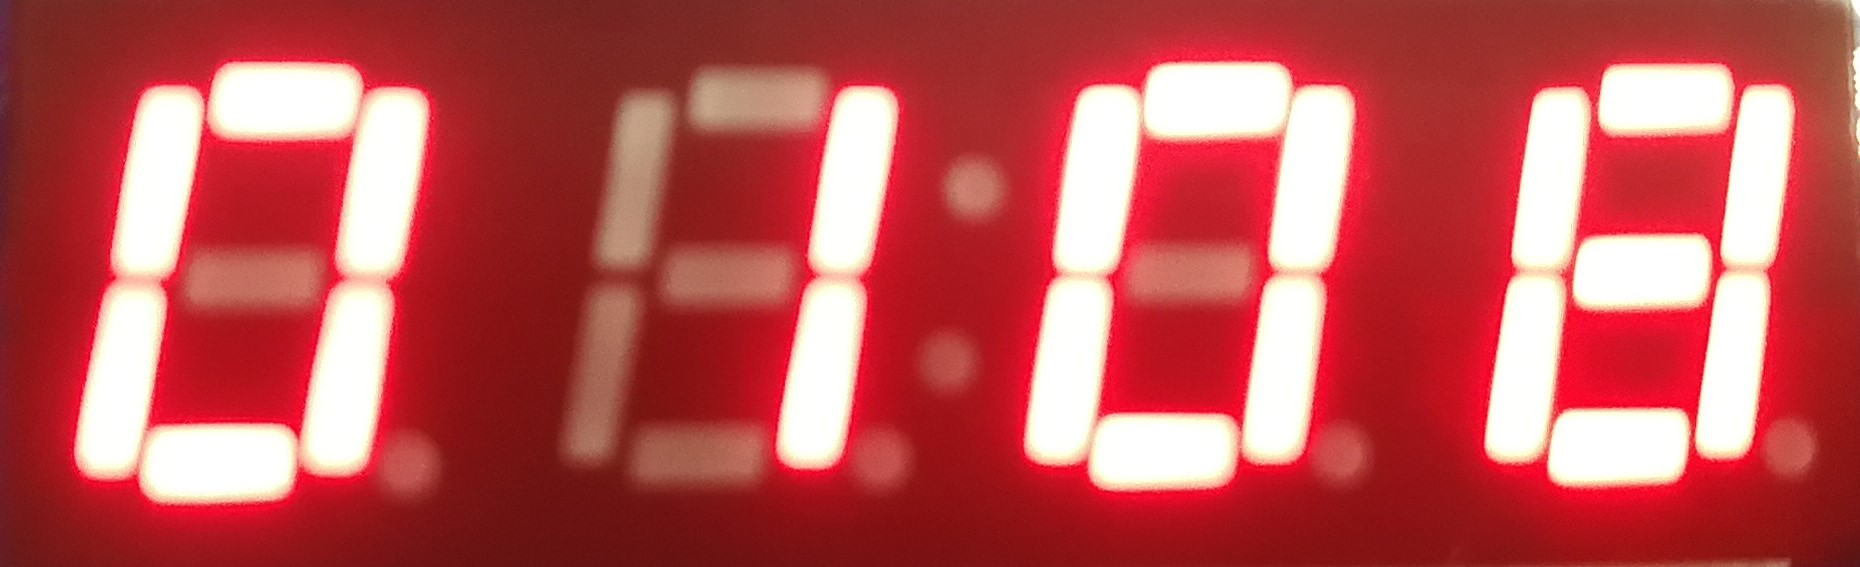
\includegraphics[width=0.3\linewidth]{fig/Implementation/0x34_01.jpg}\\
    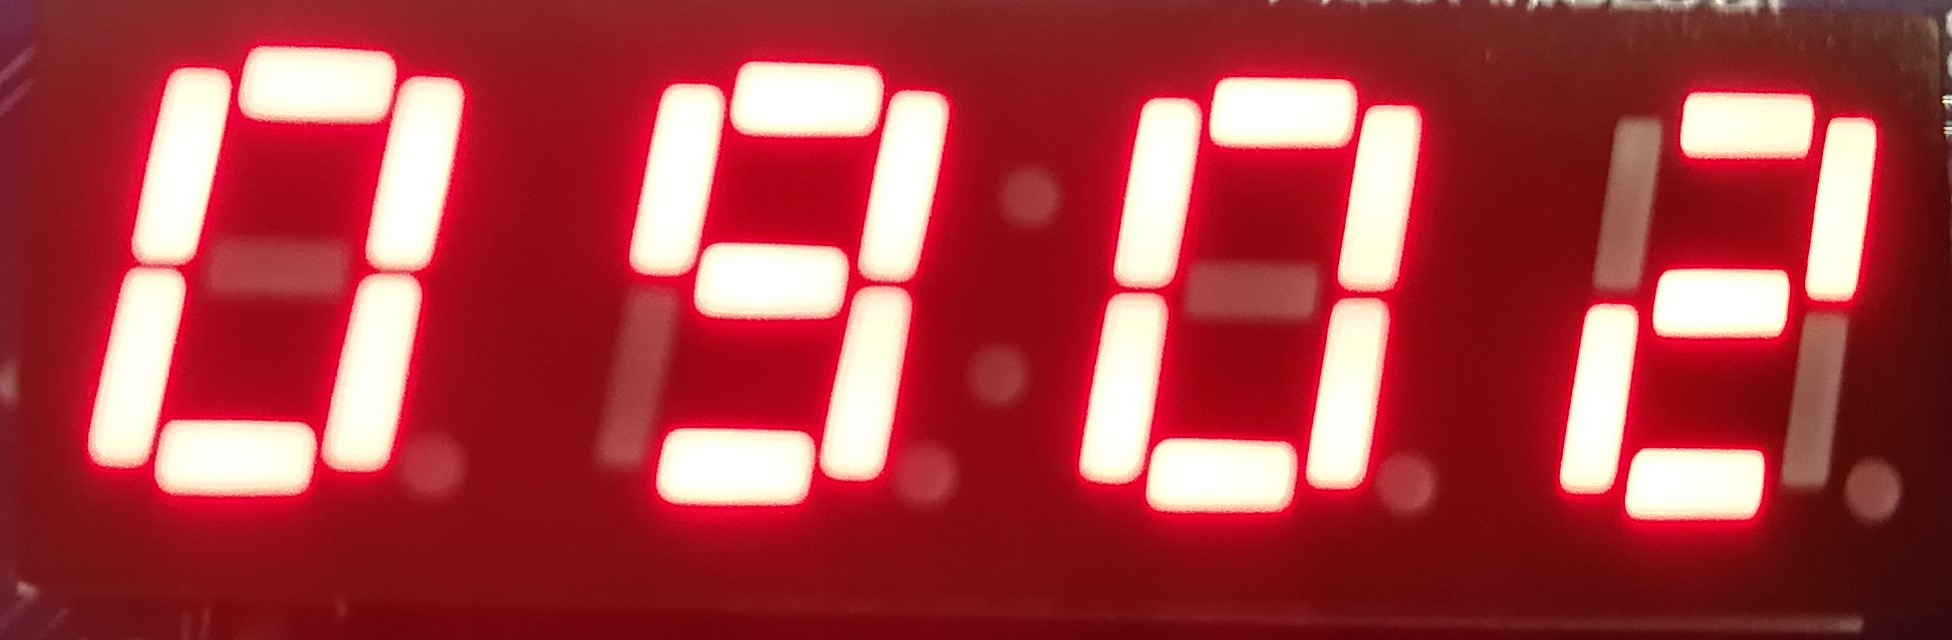
\includegraphics[width=0.3\linewidth]{fig/Implementation/0x34_10.jpg}&
    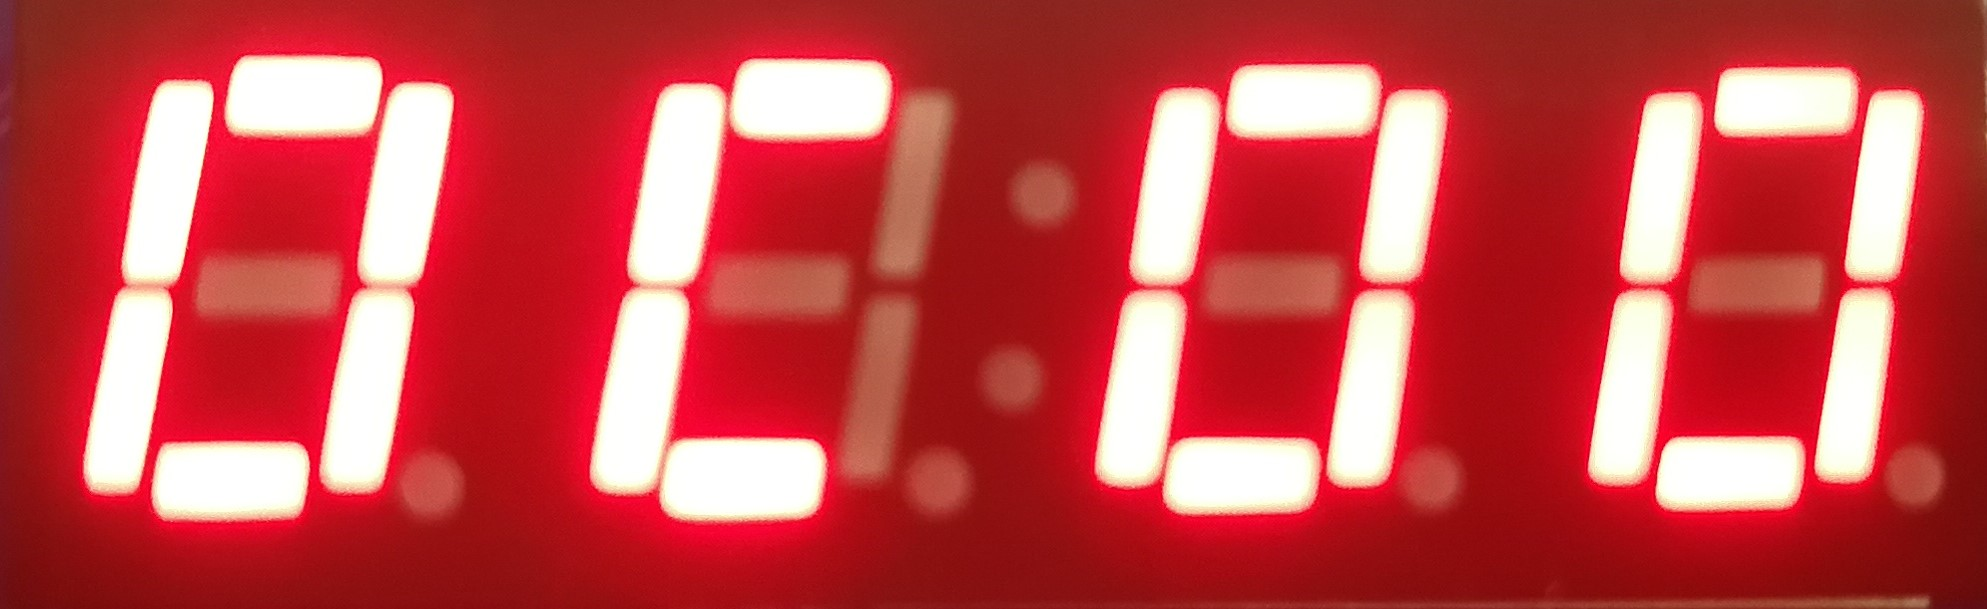
\includegraphics[width=0.3\linewidth]{fig/Implementation/0x34_11.jpg}
    \end{tabular}
    \caption{0x34结果}
    \end{figure}
\end{enumerate}